% ATLAS Build Graph: the build plan cut into work areas for people.
%
% This file is the source of documents/ATLAS_Build_Graph.pdf and is edited by hand.
% Build:  pdflatex ATLAS_Build_Graph.tex   (run it twice, for page numbers and contents)
%   or:   latexmk -pdf ATLAS_Build_Graph.tex
% The five diagrams are vector PDFs in figures/build_graph/ (drawn once from the plan's
% Mermaid diagrams). Everything else is plain LaTeX: to change a board or a table, edit
% the \card, area-table and gate-table rows below.
%
% Content follows documents/ATLAS_Master_Plan.md (sections 9 and 11.3) as of 3 October 2026.
\documentclass[10pt,a4paper,landscape]{article}
\usepackage[T1]{fontenc}
\usepackage[utf8]{inputenc}
\usepackage[a4paper,landscape,left=12mm,right=12mm,top=17mm,bottom=15mm,headheight=5mm,headsep=5mm,footskip=8mm]{geometry}
\usepackage[sfdefault,scaled=0.94,lf]{FiraSans}
\usepackage[scaled=0.82,lf]{FiraMono}
\usepackage{microtype}
\usepackage[table]{xcolor}
\usepackage{graphicx,array,tabularx,enumitem,fancyhdr,titlesec,lastpage,newunicodechar,ragged2e,multicol,fancyvrb}
\usepackage{tikz}
\usetikzlibrary{shapes.symbols}
\usepackage[most]{tcolorbox}
\usepackage[hidelinks,bookmarksnumbered,pdftitle={ATLAS Build Graph}]{hyperref}

% ---- characters that the text font does not carry
\newunicodechar{≥}{\ensuremath{\geq}}
\newunicodechar{≤}{\ensuremath{\leq}}
\newunicodechar{→}{\ensuremath{\rightarrow}}
\newunicodechar{←}{\ensuremath{\leftarrow}}
\newunicodechar{↓}{\ensuremath{\downarrow}}
\newunicodechar{−}{\ensuremath{-}}
\newunicodechar{‖}{\ensuremath{\parallel}}
\newunicodechar{φ}{\ensuremath{\varphi}}
\newunicodechar{ρ}{\ensuremath{\rho}}
\newunicodechar{κ}{\ensuremath{\kappa}}
\newunicodechar{Λ}{\ensuremath{\Lambda}}
\newunicodechar{≈}{\ensuremath{\approx}}

% ---- colours: the lanes use the colours of the plan's diagrams
\definecolor{ink}{HTML}{1D2433}
\definecolor{muted}{HTML}{4A5368}
\definecolor{rule}{HTML}{D3D7E0}
\definecolor{panel}{HTML}{F3F4F7}
\definecolor{laneAf}{HTML}{E3F4EC}\definecolor{laneAs}{HTML}{2F8F6B}\definecolor{laneAi}{HTML}{12392B}
\definecolor{laneBf}{HTML}{EEE7FB}\definecolor{laneBs}{HTML}{7B4FD6}\definecolor{laneBi}{HTML}{2C1A5C}
\definecolor{laneCf}{HTML}{FDEEDE}\definecolor{laneCs}{HTML}{D9722B}\definecolor{laneCi}{HTML}{5A2C0C}
\definecolor{laneDf}{HTML}{E3EDFC}\definecolor{laneDs}{HTML}{2B6FD9}\definecolor{laneDi}{HTML}{11305F}
\definecolor{laneXf}{HTML}{EEF1F6}\definecolor{laneXs}{HTML}{7A8499}\definecolor{laneXi}{HTML}{1D2433}

% ---- page furniture
\color{ink}
\setlength{\parindent}{0pt}
\setlength{\parskip}{1.6mm}
\setlist{nosep,leftmargin=5mm,itemsep=1mm,topsep=1mm}
\newcommand{\footline}{Follows ATLAS\_Master\_Plan.md as of 3 October 2026}
\pagestyle{fancy}
\fancyhf{}
\renewcommand{\headrule}{{\color{rule}\hrule height .4pt}}
\fancyhead[L]{\fontsize{7.5}{9}\selectfont\textbf{ATLAS Build Graph}}
\fancyhead[R]{\fontsize{7.5}{9}\selectfont\color{muted}\leftmark}
\fancyfoot[L]{\fontsize{7}{9}\selectfont\color{muted}\footline}
\fancyfoot[R]{\fontsize{7}{9}\selectfont\color{muted}Page \thepage\ of \pageref{LastPage}}
\fancypagestyle{plain}{\fancyhf{}\renewcommand{\headrule}{}%
  \fancyfoot[L]{\fontsize{7}{9}\selectfont\color{muted}\footline}%
  \fancyfoot[R]{\fontsize{7}{9}\selectfont\color{muted}Page \thepage\ of \pageref{LastPage}}}

% ---- headings; the second argument is the place in the plan, shown at the right
\titleformat{\section}[block]{\color{ink}\titlerule[1.4pt]\vspace{2.5mm}\fontsize{19}{22}\selectfont\bfseries}{\textcolor{muted}{\mdseries\thesection}}{2.5mm}{}
\titlespacing*{\section}{0pt}{0pt}{2.5mm}
\titleformat{\subsection}[block]{\fontsize{12.5}{15}\selectfont\bfseries}{\textcolor{muted}{\mdseries\thesubsection}}{2.2mm}{}
\titlespacing*{\subsection}{0pt}{3.5mm}{1.5mm}
\newcommand{\planmark}[1]{{\normalfont\fontsize{7.5}{9}\selectfont\color{muted}\if\relax\detokenize{#1}\relax\else plan #1\fi}}
\newcommand{\sect}[2]{\section[#1]{#1\hfill\planmark{#2}}\markboth{#1}{#1}}
\newcommand{\sub}[2]{\subsection[#1]{#1\hfill\planmark{#2}}}

% ---- small pieces
\newcommand{\code}[1]{{\ttfamily #1}}
\newcommand{\none}[1]{{\color{muted}#1}}
\newcommand{\ids}[1]{{\fontsize{7.5}{9.6}\selectfont\color{muted}#1}}
\newcommand{\tablefont}{\fontsize{8}{10.6}\selectfont}
\newcommand{\thinrule}{\arrayrulecolor{rule}\hline}
\newcommand{\thickrule}{\arrayrulecolor{ink}\hline}
\newcommand{\minihead}[1]{\par\smallskip\textbf{#1}\par}
\newcommand{\intro}[1]{{\fontsize{9}{12.5}\selectfont #1\par}\vspace{1.5mm}}
\newcommand{\figcap}[1]{{\fontsize{8}{11}\selectfont\color{muted}#1\par}}
\newcommand{\kicker}[1]{{\fontsize{7.5}{9}\selectfont\bfseries\color{muted}\textls[90]{\MakeUppercase{#1}}\par}\vspace{1.5mm}}
\newcommand{\lanetitle}[1]{\par\medskip{\fontsize{10}{12}\selectfont\bfseries #1\par}\nopagebreak\vspace{.5mm}}
\newcommand{\legendrow}[2]{\noindent\makebox[15mm][l]{#1}\parbox[t]{88mm}{\RaggedRight #2}\par\vspace{.6mm}}
\newcommand{\swatch}[1]{\raisebox{-1.2mm}{\tikz\draw[draw=lane#1s,fill=lane#1f,line width=.7pt] (0,0) rectangle (11mm,4.6mm);}}
\newcommand{\tocline}[2]{\noindent\hyperref[#1]{\makebox[5mm][l]{\ref*{#1}}#2}\,{\color{rule}\dotfill}\,\pageref{#1}\par\vspace{.4mm}}

% ---- an area tag such as \tg{B}{B2}, and a gate such as \gate{G3}
\newcommand{\tg}[2]{\tcbox[on line,colback=lane#1f,colframe=lane#1s,boxrule=.4pt,arc=.8pt,boxsep=0pt,left=1.6pt,right=1.6pt,top=1pt,bottom=1pt]%
  {\fontsize{6.8}{7}\selectfont\bfseries\color{lane#1i}#2}}
\newcommand{\gate}[1]{\tikz[baseline=(g.base)]\node[signal,signal to=east and west,fill=ink,text=white,inner xsep=.5pt,inner ysep=1.7pt,
  font=\fontsize{6.8}{7}\selectfont\bfseries](g){#1};}

% ---- the board: one column per lane, one row per step
%      \card{lane}{tag}{name}{after ... needs ... feeds ...}
\newcommand{\card}[4]{%
  \begin{tcolorbox}[enhanced,frame hidden,colback=lane#1f,borderline west={2pt}{0pt}{lane#1s},sharp corners,boxrule=0pt,boxsep=0pt,
      left=6pt,right=3pt,top=3pt,bottom=3pt,before skip=0pt,after skip=2.4pt]
  {\fontsize{8}{9.8}\selectfont\color{lane#1i}\RaggedRight\tg{#1}{#2}\hspace{2pt}\textbf{#3}\par}%
  \if\relax\detokenize{#4}\relax\else{\vspace{1.2pt}\fontsize{7.5}{11}\selectfont\color{ink}\RaggedRight #4\par}\fi
  \end{tcolorbox}}
\newcommand{\lanehead}[2]{%
  \begin{tcolorbox}[enhanced,frame hidden,colback=lane#1f,borderline north={2pt}{0pt}{lane#1s},sharp corners,boxrule=0pt,boxsep=0pt,
      left=5pt,right=3pt,top=5pt,bottom=3pt,before skip=0pt,after skip=0pt]
  {\fontsize{8.2}{10}\selectfont\bfseries\color{lane#1i}#2}\end{tcolorbox}}
\newcommand{\step}[1]{\vspace{2mm}{\fontsize{7.5}{9}\selectfont\color{muted}#1}}
\newenvironment{board}[1]{\par\noindent\setlength{\tabcolsep}{.8mm}\renewcommand{\arraystretch}{1}%
  \tabularx{\linewidth}{@{}>{\vspace{0pt}\centering\arraybackslash}p{7mm}*{#1}{>{\vspace{0pt}}X}@{}}}%
  {\endtabularx\par}

% ---- the tables
\newcolumntype{L}[1]{>{\RaggedRight\arraybackslash}p{#1}}
\newenvironment{areatable}{\par\noindent\tablefont\setlength{\tabcolsep}{2mm}\renewcommand{\arraystretch}{1.3}%
  \begin{tabular}{@{}L{80mm}L{24mm}L{50mm}L{50mm}L{19mm}L{28mm}@{}}
  \rowcolor{panel}\textbf{Area and what it delivers} & \textbf{Starts after} & \textbf{Also needs, before it can finish} &
  \textbf{Hands over to other lanes} & \textbf{Feeds gate} & \textbf{Inside, in the plan} \\ \thickrule}%
  {\end{tabular}\par}
\newenvironment{gatetable}{\par\noindent\tablefont\setlength{\tabcolsep}{2mm}\renewcommand{\arraystretch}{1.3}%
  \begin{tabular}{@{}L{44mm}L{90mm}L{95mm}L{30mm}@{}}
  \rowcolor{panel}\textbf{Gate} & \textbf{Needs} & \textbf{Passes when (summary)} & \textbf{Present} \\ \thickrule}%
  {\end{tabular}\par}
\newtcolorbox{quoted}{enhanced,breakable,frame hidden,colback=white,borderline west={1.2pt}{0pt}{rule},sharp corners,boxrule=0pt,
  left=4mm,right=0mm,top=0mm,bottom=0mm,boxsep=0pt,fontupper=\fontsize{9}{12.4}\selectfont}

% ---- one A3 landscape page inside the A4 document, for a diagram that would be too small on A4
\newsavebox{\bigbox}
\newenvironment{bigpage}[1]{%
  \clearpage\thispagestyle{empty}%
  \pdfpagewidth=420mm \pdfpageheight=297mm
  \begin{lrbox}{\bigbox}\begin{minipage}[t][277mm][t]{396mm}%
  \setlength{\parindent}{0pt}\setlength{\parskip}{1.6mm}%
  {\fontsize{7.5}{9}\selectfont\textbf{ATLAS Build Graph}\hfill{\color{muted}#1}\par}\vspace{-.6mm}{\color{rule}\hrule height .4pt}\vspace{3.6mm}%
}{%
  \par\vfill{\fontsize{7}{9}\selectfont\color{muted}\footline\hfill Page \thepage\ of \pageref{LastPage}\par}%
  \end{minipage}\end{lrbox}%
  \noindent\vbox to 0pt{\kern-9.5mm\hbox to 0pt{\usebox{\bigbox}\hss}\vss}%
  \clearpage}

\begin{document}

%% ======================================================================
%% Cover
%% ======================================================================
\thispagestyle{plain}
\noindent\begin{minipage}[t]{150mm}
\kicker{StormHacks 2026, team handout}
{\fontsize{34}{36}\selectfont\bfseries ATLAS Build Graph\par}
\vspace{2mm}
{\fontsize{13}{17}\selectfont\color{muted}Who builds what, what can run side by side, what has to wait, and the gates in between.\par}
\vspace{7mm}
{\fontsize{10.5}{15}\selectfont This is the build plan cut for people. Each box is one area of work that one person owns, about the
size of ``implement hyperbolic terrain generation'', not a single task. For every phase it shows the areas of each lane, which
of them can start at the same time, which one waits for another, what is handed from one person to the next, and the gate
each area feeds.\par}
\vspace{3mm}
Everything here follows \code{documents/ATLAS\_Master\_Plan.md} as it stood on 3 October 2026. The work areas are the ones the plan
defines (§9.5.2 for Phase 1, ``Work areas'' in §9.6 to §9.8); who waits for whom follows from the dependencies of the tasks
inside each area. The tasks themselves, with their outputs and acceptance tests, stay in the plan (§9 and §10) for the coding
agents. Work is ordered by dependencies and gates only.\par
\vspace{6mm}
\kicker{How to read an area}
\begin{itemize}
  \item \textbf{Starts after} (on the boards: \textbf{after}): nothing inside the area can begin until the named area or gate is done.
  \item \textbf{Also needs} (\textbf{needs}): the area can start, but one part of it waits for something from another area.
  \item \textbf{Feeds}: the gates at which the area's work is checked.
  \item \textbf{Hands over to}: what another lane is waiting for from this area. These are the moments to talk.
  \item A tag such as \tg{B}{B2} is lane B, second area of that phase. Task ids such as \code{P1-B04} (phase 1, lane B,
        number 04) only point into the plan. Gates are G0 to G15.
\end{itemize}
\end{minipage}\hfill
\begin{minipage}[t]{105mm}
\kicker{Legend}
\legendrow{\swatch{A}}{\textbf{Lane A} · Platform, Look and Flat Spaces}
\legendrow{\swatch{B}}{\textbf{Lane B} · Kernel and Curved Worlds}
\legendrow{\swatch{C}}{\textbf{Lane C} · Scan, Room and Safety}
\legendrow{\swatch{D}}{\textbf{Lane D} · Link, Station and Forge}
\legendrow{\swatch{X}}{\textbf{All hands} · shared work}
\legendrow{\gate{G0}}{\textbf{Gate} · where the lanes meet and a check is passed}
\legendrow{$\longrightarrow$}{\textbf{Arrow} · the area at its head needs something from the area at its tail}
\vspace{6mm}
\kicker{Contents}
\tocline{sec:big}{The big picture}
\tocline{sec:p1}{Phase 1 · Foundation}
\tocline{sec:p2}{Phase 2 · Geometry Playground and Lung Mission}
\tocline{sec:p3}{Phase 3 · Shared House and FieldFit}
\tocline{sec:p4}{Phase 4 · Finish}
\tocline{sec:rules}{Ground rules}
\end{minipage}

%% ======================================================================
%% 1  The big picture (A3 page: gates diagram and the lanes table)
%% ======================================================================
\begin{bigpage}{The big picture}
\sect{The big picture}{}\label{sec:big}
\sub{Phases and gates}{§9.4}
\centerline{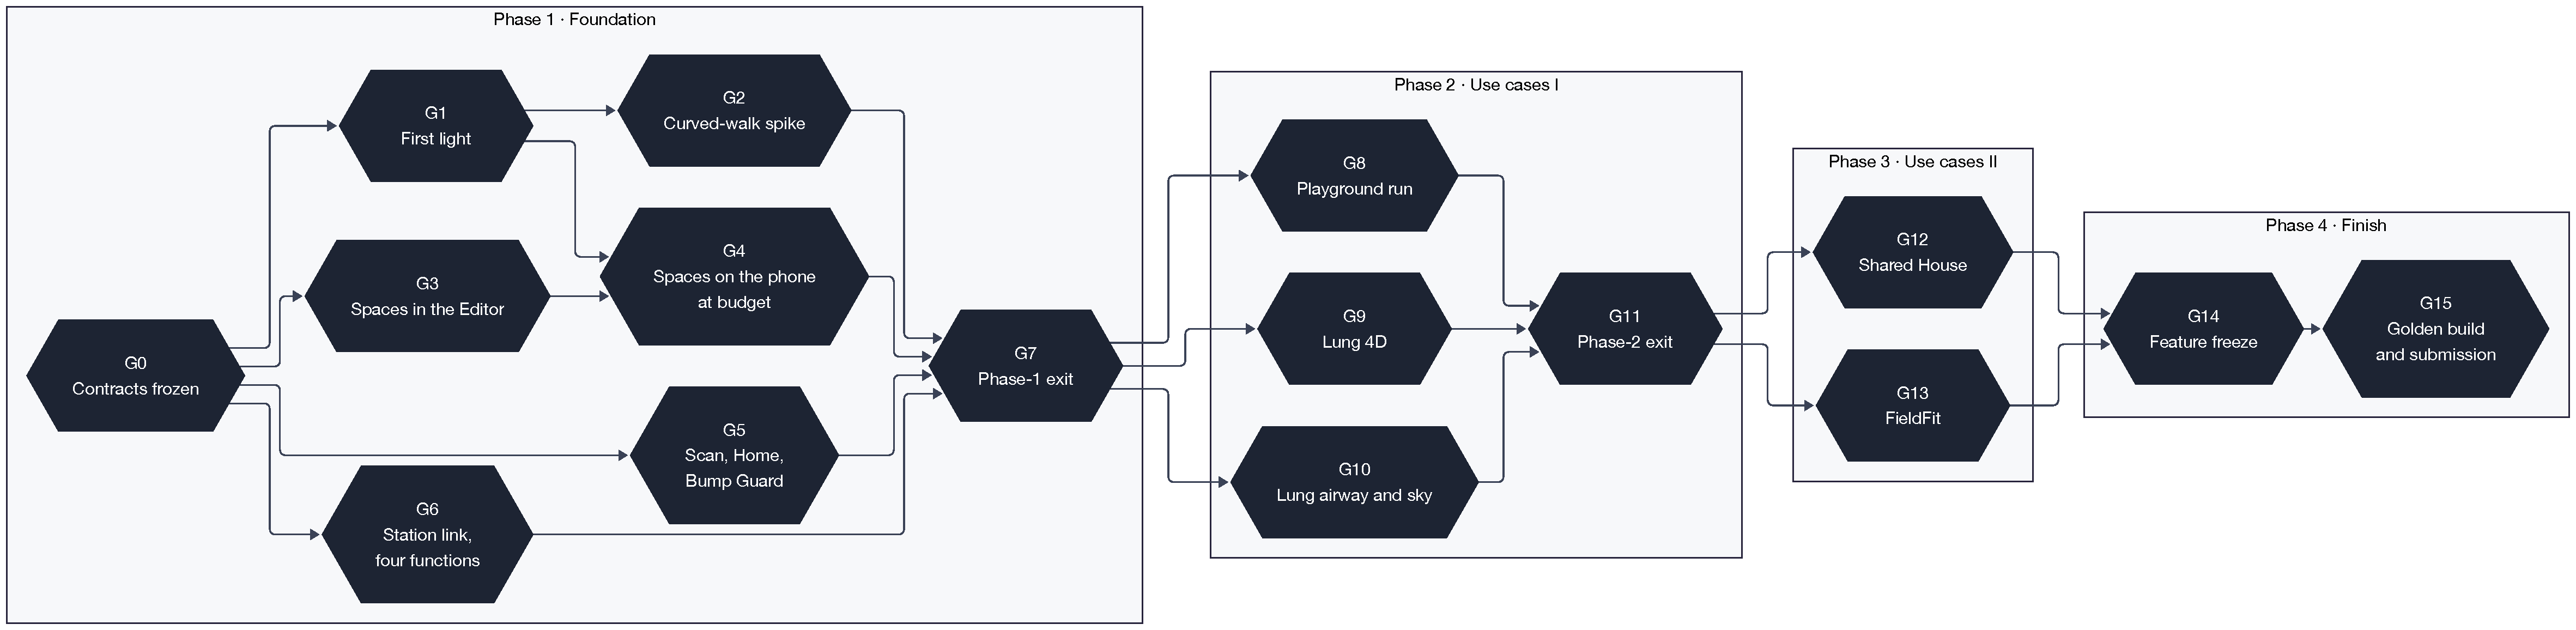
\includegraphics[width=390mm,height=110mm,keepaspectratio]{figures/build_graph/gates.pdf}}
\smallskip
Phase 3's packages depend technically only on Phase 1. They are placed after G11 because every lane is occupied until then.\par

\sub{The four lanes: who owns what}{§9.2}
{\tablefont\renewcommand{\arraystretch}{1.3}\setlength{\tabcolsep}{2mm}\begin{tabularx}{\linewidth}{@{}>{\RaggedRight\arraybackslash}X >{\RaggedRight\arraybackslash}X >{\RaggedRight\arraybackslash}X >{\RaggedRight\arraybackslash}X >{\RaggedRight\arraybackslash}X@{}}
\rowcolor{panel}\textbf{Lane} & \textbf{Phase 1 · Foundation} & \textbf{Phase 2 · Use cases I} & \textbf{Phase 3 · Use cases II} & \textbf{Phase 4 · Finish} \\ \thickrule
\cellcolor{laneAf}\color{laneAi}\textbf{A · Platform, Look and Flat Spaces} & Project, build seat, stereo rig, lens blit, shared shader, SpaceLab, Glued (S1), Impossible Rooms (S5), Slicer and \code{Mesh4D} (S6), room content in Glued, thermal ladder, soak & Slicer toybox, equation sources, look of the Playground; the whole medical 4D runtime (worldtube, breath lane, scanner tilt, tasks) and the Lung director with its labels and credits & Shared House: sheets, door, second home, visitor & Look and audio, performance hardening, golden build \\ \thinrule
\cellcolor{laneBf}\color{laneBi}\textbf{B · Kernel and Curved Worlds} & Kernel, holonomy rig, warp shader, exact tile ids, tile meshes and renderer, world generator, Small Planet (S4), dial and 3-4-5 walk, Aligned Cells (S3), room as tile zero, room content in Aligned Cells & Lung Mission: airway wing in hyperbolic space, valve chambers, Two Compasses, needle sky & FieldFit: lens mathematics, lookup, composed final blit, blind-spot finder & Maths notes, correctness report, equation-card audit, figures \\ \thinrule
\cellcolor{laneCf}\color{laneCi}\textbf{C · Scan, Room and Safety} & AR session, FloorScan core (Editor), scan routes, RoomModel and loop-fit, Home (S0), object photos, Bump Guard with its warning cue and haptics, input, pose pipeline, onboarding, pre-scan path & Geometry Playground: the shell (director, guided walk, captions, twins, menu), the pointing probe, and the Glued and Impossible Rooms exhibits & Shared House: second scan, door fit, Bump Guard on the second sheet, peer link & Onboarding with outside walkers, comfort protocol, failure drills, rehearsals \\ \thinrule
\cellcolor{laneDf}\color{laneDi}\textbf{D · Link, Station and Forge} & \code{Atlas.\allowbreak{}Link}, Hub, tuner and Console, perf probe and telemetry, Spectator, flat-twin map, Forge and mesh clean-up, asset client, built-in fallback set, on-device menu, pairing & Lung Mission: the Station pipeline (\code{atlas case}), case packages, plan card, Lung panels on Console and Spectator & FieldFit: field presets, Console lens panel, Spectator heatmap, search task and logging; Shared House: peer relay (Extended) and two-plan flat twin & Judges' dashboard, session logs, metrics report, video capture, deck \\ \thinrule
Work packages & A 15 · B 12 · C 15 · D 13 (+ 8 shared, 7 gates) & A 17 · B 12 · C 17 · D 13 & A 7 · B 8 · C 5 · D 8 & A 5 · B 5 · C 6 · D 6 \\ \thinrule
\end{tabularx}\par}

The lane owner decides inside the lane. Anything that touches a contract (§6.4) is announced to all four before it is committed.\par
\end{bigpage}


%% ======================================================================
%% Phase 1 · Foundation
%% ======================================================================

\clearpage\sect{Phase 1 · Foundation}{§9.5}\label{sec:p1}

\sub{Who can work side by side}{}

\intro{This phase opens the build. 17 areas cover the 63 tasks of this phase. Across a row: areas that can be worked on at the same point. Down a column: one person's order. An area sits in the first step in which part of it can begin; it is finished only when everything under \emph{after} and \emph{needs} has arrived.}

\begin{board}{4}
 & \lanehead{A}{Lane A · Platform, Look and Flat Spaces} & \lanehead{B}{Lane B · Kernel and Curved Worlds} & \lanehead{C}{Lane C · Scan, Room and Safety} & \lanehead{D}{Lane D · Link, Station and Forge} \\[1mm]
\step{1} & \multicolumn{4}{@{}p{\dimexpr\linewidth-9.4mm\relax}@{}}{\vspace{0pt}\card{X}{All}{The start: set-up and contracts}{feeds \gate{G0}}} \\
\step{2} &
  \card{A}{A1}{Get the app running in stereo on both phones}{after \tg{X}{All} \quad feeds \gate{G1}} &
  \card{B}{B1}{Implement the geometry kernel and the curved-walk rig}{after \tg{X}{All} \quad needs \gate{G0} \quad feeds \gate{G2}} &
  \card{C}{C2}{Implement room scanning and the RoomModel}{after \tg{X}{All} \quad needs \gate{G0}\,\tg{C}{C1}} &
  \card{D}{D1}{Build the phone-to-Station link}{after \tg{X}{All} \quad needs \tg{A}{A1} \quad feeds \gate{G1}}\card{D}{D4}{Build the Forge: object photos to furniture meshes}{after \tg{X}{All} \quad needs \tg{C}{C3}\,\tg{D}{D1} \quad feeds \gate{G6}} \\[.6mm]
\step{3} &
  \card{A}{A2}{Build the shared look shader and the SpaceLab host}{after \gate{G0}\,\tg{A}{A1}} &
  \card{B}{B2}{Implement hyperbolic terrain generation}{after \tg{B}{B1} \quad needs \gate{G0}\,\tg{A}{A2} \quad feeds \gate{G3}\,\gate{G6}} &
  \card{C}{C1}{Bring up AR tracking, input and the pose pipeline}{after \tg{A}{A1} \quad needs \tg{A}{A2} \quad feeds \gate{G1}\,\gate{G2}\,\gate{G5}} &
  \card{D}{D2}{Build live tuning, the operator Console and telemetry}{after \tg{D}{D1} \quad needs \tg{A}{A1}\,\tg{C}{C1}\,\tg{C}{C3} \quad feeds \gate{G1}\,\gate{G5}\,\gate{G6}} \\[.6mm]
\step{4} &
  \card{A}{A3}{Implement the flat and 4D spaces}{after \tg{A}{A2} \quad needs \tg{C}{C3} \quad feeds \gate{G3}\,\gate{G7}} &
   &
  \card{C}{C3}{Rebuild the room as Home and add Bump Guard}{after \tg{C}{C1} \quad needs \gate{G0}\,\tg{A}{A2}\,\tg{C}{C2} \quad feeds \gate{G5}\,\gate{G6}} &
  \card{D}{D3}{Build the Spectator mirror and the flat-twin map}{after \tg{A}{A2}\,\tg{D}{D1} \quad needs \tg{B}{B2} \quad feeds \gate{G6}} \\[.6mm]
\step{5} &
   &
  \card{B}{B3}{Implement Small Planet and Aligned Cells}{after \gate{G0}\,\tg{B}{B2} \quad needs \tg{C}{C3} \quad feeds \gate{G3}\,\gate{G7}} &
  \card{C}{C4}{Build onboarding and the pre-scan path}{after \tg{C}{C2} \quad needs \tg{C}{C3}\,\tg{D}{D1} \quad feeds \gate{G5}} &
   \\[.6mm]
\step{6} &
  \card{A}{A4}{Hold the frame rate: thermal ladder, performance runs and soak}{after \tg{C}{C3}\,\tg{D}{D2} \quad needs \gate{G3}\,\tg{A}{A3}\,\tg{B}{B3}\,\tg{B}{B4} \quad feeds \gate{G4}} &
  \card{B}{B4}{Put the scanned room into the curved world}{after \tg{B}{B2}\,\tg{C}{C2} \quad needs \tg{B}{B3}\,\tg{C}{C3} \quad feeds \gate{G7}} &
   &
   \\[.6mm]
\end{board}


\begin{bigpage}{Phase 1 · Foundation}
\sub{The work areas, as the plan draws them}{§9.5.2}
Sixteen work areas, a handful per lane. An area is the unit a person plans in, about the size of "Implement hyperbolic terrain generation" or "Build the Forge: object photos to furniture meshes"; the tasks inside it (§9.5.4 onwards) are the units handed to agents. An arrow means the area at its head needs something from the area at its tail.\par\medskip
\centerline{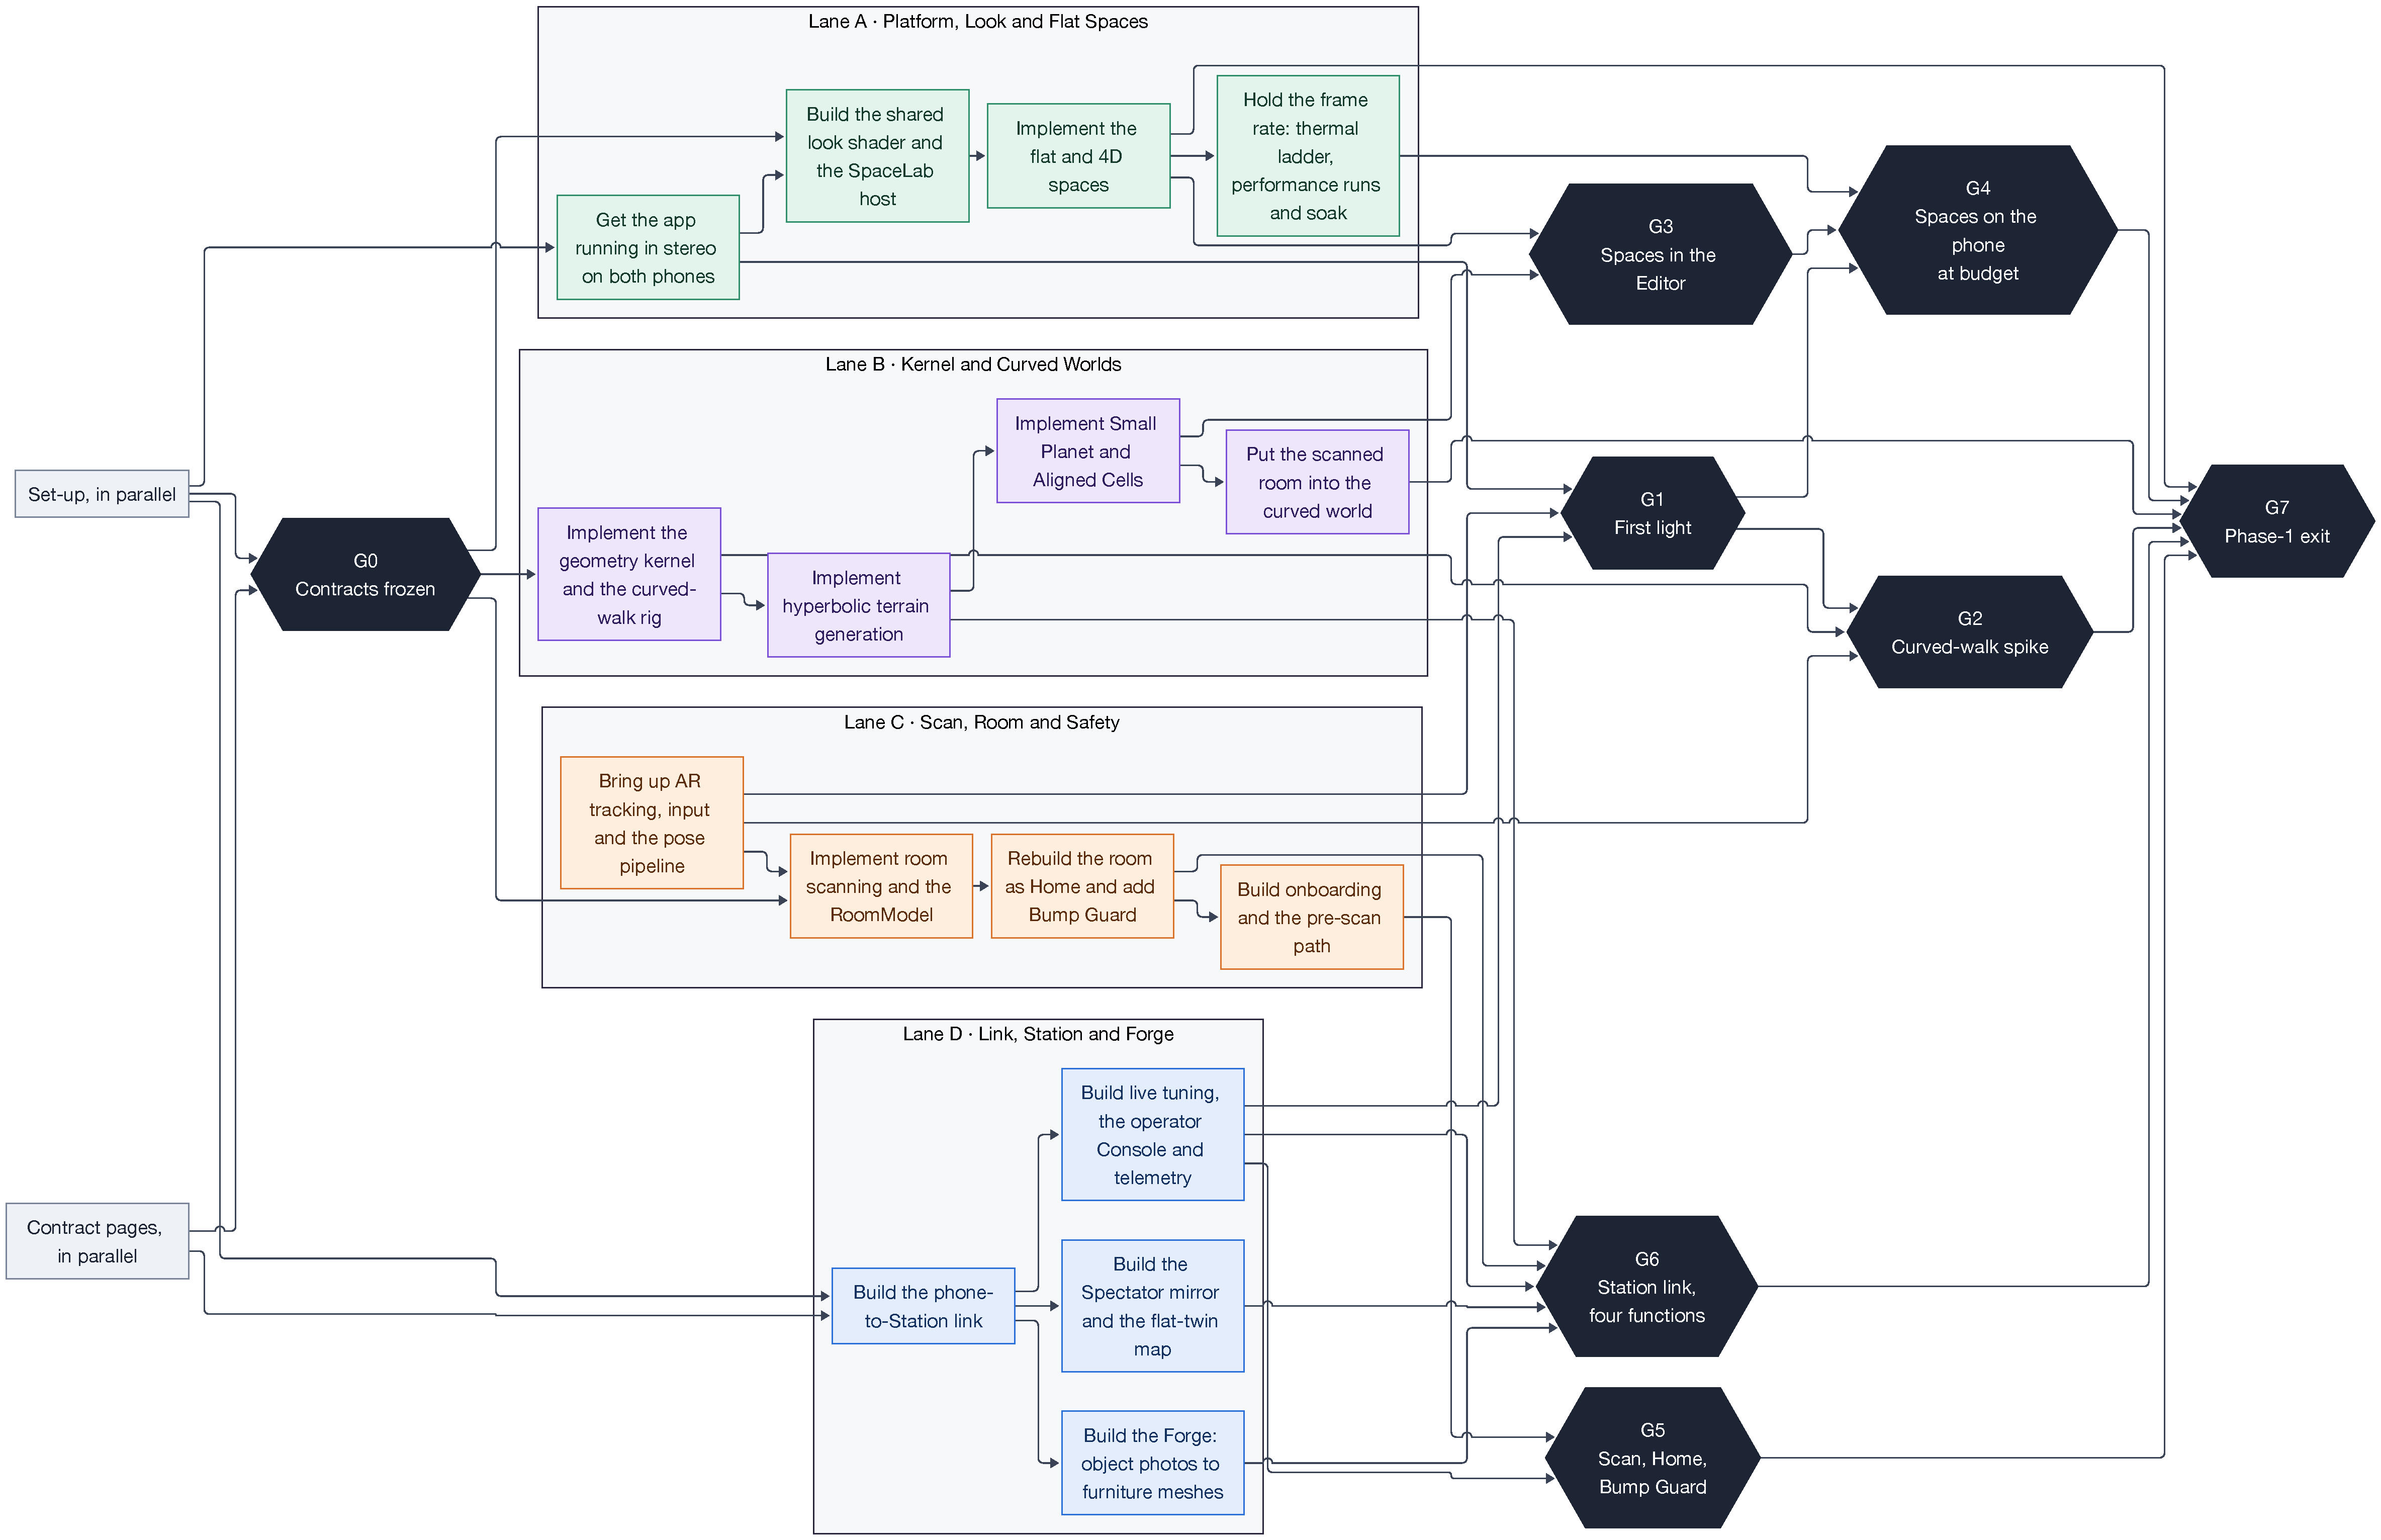
\includegraphics[width=392mm,height=215mm,keepaspectratio]{figures/build_graph/phase1_areas.pdf}}
\medskip
\figcap{Each box shows the name of the area; what it covers is in the tables that follow.}
\end{bigpage}

\clearpage
\sub{The areas, lane by lane}{}
\lanetitle{All hands}
\begin{areatable}
  \tg{X}{All} \textbf{The start: set-up and contracts}\newline Build seat, signing and Unity (lane A leads, everyone takes part); Contracts frozen (this is gate G0); Station ready (lane D); Phones and network ready (lane C); Contract pages, lane A; Contract pages, lane B; Contract pages, lane C; Contract pages, lane D; Unity project and repository skeleton.
  & \none{nothing in this phase}
  & \none{--}
  & \tg{A}{A1} Unity project and repository skeleton; Phones and network ready (lane C)\newline \tg{B}{B1} Unity project and repository skeleton\newline \tg{C}{C2} Unity project and repository skeleton; Contract pages, lane C\newline \tg{D}{D1} Contract pages, lane D; Station ready (lane D)\newline \tg{D}{D4} Station ready (lane D); Contract pages, lane D
  & \gate{G0}
  & \ids{9 tasks: P1-X01, X02, X03, X04, X05, X06, X07, X08, A01} \\ \thinrule
\end{areatable}

\lanetitle{Lane A · Platform, Look and Flat Spaces}
\begin{areatable}
  \tg{A}{A1} \textbf{Get the app running in stereo on both phones}\newline the first build on both phones, URP settings and quality tiers, the two-camera stereo rig, the lens pre-distortion blit, and a one-command build
  & \tg{X}{All}
  & \none{--}
  & \tg{C}{C1} First build on both phones; Two-camera stereo rig\newline \tg{C}{C3} Two-camera stereo rig\newline \tg{D}{D1} First build on both phones\newline \tg{D}{D2} Two-camera stereo rig
  & \gate{G1}
  & \ids{5 tasks: P1-A02, A03, A04, A05, A13} \\ \thinrule
  \tg{A}{A2} \textbf{Build the shared look shader and the SpaceLab host}\newline the one shader and palette that every space uses, and the boot scene that loads one space at a time and runs the frame loop
  & \gate{G0} \tg{A}{A1}
  & \none{--}
  & \tg{B}{B2} Shared look shader\newline \tg{C}{C1} SpaceLab host\newline \tg{C}{C3} Shared look shader\newline \tg{D}{D3} Shared look shader; SpaceLab host
  & \none{--}
  & \ids{2 tasks: P1-A06, A08} \\ \thinrule
  \tg{A}{A3} \textbf{Implement the flat and 4D spaces}\newline the Glued space (S1) with the scanned room in it, the stencil portal engine and Impossible Rooms (S5), and the Slicer (S6) with Mesh4D
  & \tg{A}{A2}
  & \tg{C}{C3} Home rebuild S0
  & \none{--}
  & \gate{G3} \gate{G7}
  & \ids{5 tasks: P1-A09, A10, A11, A12, A15} \\ \thinrule
  \tg{A}{A4} \textbf{Hold the frame rate: thermal ladder, performance runs and soak}\newline the thermal quality ladder, a performance run for every space on the budget fixture, and the soak
  & \tg{C}{C3} \tg{D}{D2}
  & \gate{G3}\newline \tg{A}{A3} Room content in Glued, and standing mode\newline \tg{B}{B3} Room content in Aligned Cells\newline \tg{B}{B4} The room becomes tile zero
  & \none{--}
  & \gate{G4}
  & \ids{2 tasks: P1-A07, A14} \\ \thinrule
\end{areatable}

\lanetitle{Lane B · Kernel and Curved Worlds}
\begin{areatable}
  \tg{B}{B1} \textbf{Implement the geometry kernel and the curved-walk rig}\newline the double-precision kernel for hyperbolic, flat and spherical space, and the holonomy rig that turns head movement into movement through curved space
  & \tg{X}{All}
  & \gate{G0}
  & \none{--}
  & \gate{G2}
  & \ids{2 tasks: P1-B01, B02} \\ \thinrule
  \tg{B}{B2} \textbf{Implement hyperbolic terrain generation}\newline the warp shader, exact tile ids and the tile graph, procedural tile meshes, the tile renderer, and the world generator with WorldLint
  & \tg{B}{B1}
  & \gate{G0}\newline \tg{A}{A2} Shared look shader
  & \tg{D}{D3} Exact tile ids and the tile graph
  & \gate{G3} \gate{G6}
  & \ids{5 tasks: P1-B03, B04, B05, B06, B07} \\ \thinrule
  \tg{B}{B3} \textbf{Implement Small Planet and Aligned Cells}\newline the spherical space (S4) and the flat-cell mode of the hyperbolic world (S3, Mode 2), with the scanned room in it
  & \gate{G0} \tg{B}{B2}
  & \tg{C}{C3} Home rebuild S0
  & \tg{A}{A4} Room content in Aligned Cells
  & \gate{G3} \gate{G7}
  & \ids{3 tasks: P1-B08, B10, B12} \\ \thinrule
  \tg{B}{B4} \textbf{Put the scanned room into the curved world}\newline the curvature dial, the 3-4-5 walk, and the scanned room as tile zero of the curved world
  & \tg{B}{B2} \tg{C}{C2}
  & \tg{B}{B3} Small Planet S4\newline \tg{C}{C3} Home rebuild S0
  & \tg{A}{A4} The room becomes tile zero
  & \gate{G7}
  & \ids{2 tasks: P1-B09, B11} \\ \thinrule
\end{areatable}

\lanetitle{Lane C · Scan, Room and Safety}
\begin{areatable}
  \tg{C}{C1} \textbf{Bring up AR tracking, input and the pose pipeline}\newline the AR session with Editor simulation and replay, gamepad and gaze input with twins, and the pose pipeline
  & \tg{A}{A1}
  & \tg{A}{A2} SpaceLab host
  & \tg{D}{D2} Input and twins
  & \gate{G1} \gate{G2} \gate{G5}
  & \ids{3 tasks: P1-C01, C10, C11} \\ \thinrule
  \tg{C}{C2} \textbf{Implement room scanning and the RoomModel}\newline the FloorScan core, the manual and automatic scan routes, object boxes, the RoomPlan wall bridge (Extended), and the RoomModel with the loop-fit
  & \tg{X}{All}
  & \gate{G0}\newline \tg{C}{C1} AR session and Editor simulation
  & \tg{B}{B4} RoomModel and the loop-fit
  & \none{--}
  & \ids{6 tasks: P1-C02, C03, C04, C05, C06, C15} \\ \thinrule
  \tg{C}{C3} \textbf{Rebuild the room as Home and add Bump Guard}\newline the Home rebuild (S0), object photo capture for the Forge, the warning cue and haptics, and Bump Guard
  & \tg{C}{C1}
  & \gate{G0}\newline \tg{A}{A2} Shared look shader\newline \tg{C}{C2} RoomModel and the loop-fit; Object boxes
  & \tg{A}{A3} Home rebuild S0\newline \tg{A}{A4} Home rebuild S0\newline \tg{B}{B3} Home rebuild S0\newline \tg{B}{B4} Home rebuild S0\newline \tg{D}{D2} Warning cue and haptics\newline \tg{D}{D4} Home rebuild S0
  & \gate{G5} \gate{G6}
  & \ids{4 tasks: P1-C07, C08, C09, C14} \\ \thinrule
  \tg{C}{C4} \textbf{Build onboarding and the pre-scan path}\newline onboarding with the phone in the hand, and a saved world map that relocalises in a room scanned earlier
  & \tg{C}{C2}
  & \tg{C}{C3} Home rebuild S0\newline \tg{D}{D1} Pairing and network bring-up
  & \none{--}
  & \gate{G5}
  & \ids{2 tasks: P1-C12, C13} \\ \thinrule
\end{areatable}

\lanetitle{Lane D · Link, Station and Forge}
\begin{areatable}
  \tg{D}{D1} \textbf{Build the phone-to-Station link}\newline the Atlas.Link library, the Hub, and pairing and network bring-up
  & \tg{X}{All}
  & \tg{A}{A1} First build on both phones
  & \tg{C}{C4} Pairing and network bring-up
  & \gate{G1}
  & \ids{3 tasks: P1-D01, D02, D11} \\ \thinrule
  \tg{D}{D2} \textbf{Build live tuning, the operator Console and telemetry}\newline the parameter registry and Console tuner, the operator Console, the on-device menu, and the perf probe, HUD and telemetry
  & \tg{D}{D1}
  & \tg{A}{A1} Two-camera stereo rig\newline \tg{C}{C1} Input and twins\newline \tg{C}{C3} Warning cue and haptics
  & \tg{A}{A4} Perf probe, HUD and telemetry; Operator Console
  & \gate{G1} \gate{G5} \gate{G6}
  & \ids{4 tasks: P1-D03, D04, D06, D13} \\ \thinrule
  \tg{D}{D3} \textbf{Build the Spectator mirror and the flat-twin map}\newline the Spectator build that re-renders the walker's view on the Station, and the flat-twin mini-map
  & \tg{A}{A2} \tg{D}{D1}
  & \tg{B}{B2} Exact tile ids and the tile graph
  & \none{--}
  & \gate{G6}
  & \ids{2 tasks: P1-D05, D07} \\ \thinrule
  \tg{D}{D4} \textbf{Build the Forge: object photos to furniture meshes}\newline the Forge service on the Station, mesh clean-up, the asset client on the phone, and the built-in fallback set
  & \tg{X}{All}
  & \tg{C}{C3} Home rebuild S0\newline \tg{D}{D1} Atlas.Link library
  & \none{--}
  & \gate{G6}
  & \ids{4 tasks: P1-D08, D09, D10, D12} \\ \thinrule
\end{areatable}

\sub{Gates of this phase}{§9.4}
\begin{gatetable}
  \gate{G0} \textbf{Contracts frozen} & \tg{X}{All} The start: set-up and contracts & Every contract of §6.4 is written and stubbed; each lane's sandbox runs against the stubs & all four lanes \\ \thinrule
  \gate{G1} \textbf{First light} & \tg{A}{A1} Get the app running in stereo on both phones\newline \tg{C}{C1} Bring up AR tracking, input and the pose pipeline\newline \tg{D}{D1} Build the phone-to-Station link\newline \tg{D}{D2} Build live tuning, the operator Console and telemetry\newline \gate{G0} & Empty stereo scene at 60 fps on the phone; telemetry visible on the Station; anyone can install a build & A, C, D \\ \thinrule
  \gate{G2} \textbf{Curved-walk spike} & \tg{B}{B1} Implement the geometry kernel and the curved-walk rig\newline \tg{C}{C1} Bring up AR tracking, input and the pose pipeline\newline \gate{G1} & Five-corner loop closes within 0.25 m and three walkers from the team are comfortable at the loop-fit curvature (with a spotter: Bump Guard does not exist yet). Decides the default mode and the comfort floor & B, C, three walkers from the team, a spotter \\ \thinrule
  \gate{G3} \textbf{Spaces in the Editor} & \tg{A}{A3} Implement the flat and 4D spaces\newline \tg{B}{B2} Implement hyperbolic terrain generation\newline \tg{B}{B3} Implement Small Planet and Aligned Cells\newline \gate{G0} & S1–S6 run in SpaceLab on the three sample rooms; all mathematics tests green & A, B \\ \thinrule
  \gate{G4} \textbf{Spaces on the phone at budget} & \tg{A}{A4} Hold the frame rate: thermal ladder, performance runs and soak\newline \gate{G1} \gate{G3} & Every space S0–S6 meets the Must column cold, with the room's content, on the \code{budget\_\allowbreak{}room} fixture; the 15-minute soak passes & A, B, D \\ \thinrule
  \gate{G5} \textbf{Scan, Home and Bump Guard} & \tg{C}{C1} Bring up AR tracking, input and the pose pipeline\newline \tg{C}{C3} Rebuild the room as Home and add Bump Guard\newline \tg{C}{C4} Build onboarding and the pre-scan path\newline \tg{D}{D2} Build live tuning, the operator Console and telemetry\newline \gate{G0} & Both scan paths end in a registered Home; Bump Guard passes its scripted test in the headset & C, B, D \\ \thinrule
  \gate{G6} \textbf{Station link, four functions} & \tg{B}{B2} Implement hyperbolic terrain generation\newline \tg{C}{C3} Rebuild the room as Home and add Bump Guard\newline \tg{D}{D2} Build live tuning, the operator Console and telemetry\newline \tg{D}{D3} Build the Spectator mirror and the flat-twin map\newline \tg{D}{D4} Build the Forge: object photos to furniture meshes\newline \gate{G0} & Mirror, tuning and Console, telemetry, and the scan and asset round-trip all pass §7.6 & D plus one engineer from each other lane \\ \thinrule
  \gate{G7} \textbf{Phase-1 exit} & \tg{A}{A3} Implement the flat and 4D spaces\newline \tg{B}{B3} Implement Small Planet and Aligned Cells\newline \tg{B}{B4} Put the scanned room into the curved world\newline \gate{G2} \gate{G4} \gate{G5} \gate{G6} & A first-time walker goes from self-scan to every space, watched and tuned from the Station & all four lanes \\ \thinrule
\end{gatetable}

%% ======================================================================
%% Phase 2 · Geometry Playground and Lung Mission
%% ======================================================================

\clearpage\sect{Phase 2 · Geometry Playground and Lung Mission}{§9.6}\label{sec:p2}

\sub{Who can work side by side}{}

\intro{This phase opens when \gate{G7} Phase-1 exit has passed. 16 areas cover the 59 tasks of this phase. Across a row: areas that can be worked on at the same point. Down a column: one person's order. An area sits in the first step in which part of it can begin; it is finished only when everything under \emph{after} and \emph{needs} has arrived.}

\begin{board}{4}
 & \lanehead{A}{Lane A · Platform, Look and Flat Spaces} & \lanehead{B}{Lane B · Kernel and Curved Worlds} & \lanehead{C}{Lane C · Scan, Room and Safety} & \lanehead{D}{Lane D · Link, Station and Forge} \\[1mm]
\step{1} &
  \card{A}{A1}{Build the Slicer toybox exhibit}{} &
  \card{B}{B1}{Generate the airway wing in hyperbolic space}{needs \tg{D}{D2}} &
  \card{C}{C1}{Build the Geometry Playground shell and guided walk}{}\card{C}{C3}{Build the Glued and Impossible Rooms exhibits}{} &
  \card{D}{D1}{Define the case contract and the illustrative case}{}\card{D}{D3}{Build the Lung panels, plan card and event logging}{needs \tg{D}{D1}\,\tg{D}{D2} \quad feeds \gate{G10}} \\[.6mm]
\step{2} &
  \card{A}{A2}{Wire the equation sources and finish the Playground look}{after \tg{A}{A1}\,\tg{C}{C3} \quad needs \tg{C}{C2}}\card{A}{A3}{Implement the breathing-tumour 4D views}{after \tg{D}{D1} \quad needs \tg{D}{D2}} &
   &
  \card{C}{C2}{Build captions, equation cards, action twins and the exhibit menu}{after \tg{C}{C1} \quad needs \tg{A}{A1}\,\tg{C}{C3}} &
  \card{D}{D2}{Build the real-case pipeline}{after \tg{D}{D1}} \\[.6mm]
\step{3} &
  \card{A}{A4}{Build the breath lane, gating and scanner tilt}{after \tg{A}{A3}} &
  \card{B}{B3}{Build airway navigation: beacon, endoluminal window and Two Compasses}{after \tg{D}{D2} \quad needs \tg{B}{B1}\,\tg{B}{B2} \quad feeds \gate{G10}}\card{B}{B4}{Build the needle sky}{after \tg{D}{D2} \quad feeds \gate{G10}} &
  \card{C}{C4}{Check Bump Guard in every space and run the Playground}{after \tg{A}{A2} \quad needs \tg{C}{C1}\,\tg{C}{C2} \quad feeds \gate{G8}} &
   \\[.6mm]
\step{4} &
  \card{A}{A5}{Build the Lung tasks and director, and pass the 4D soak}{after \tg{A}{A4} \quad needs \tg{D}{D2} \quad feeds \gate{G9}\,\gate{G10}} &
  \card{B}{B2}{Implement walking the airway: valve chambers and mode switch}{after \tg{B}{B1} \quad needs \tg{A}{A4} \quad feeds \gate{G10}} &
   &
   \\[.6mm]
\end{board}


\begin{bigpage}{Phase 2 · Geometry Playground and Lung Mission}
\sub{The work areas, as the plan draws them}{§9.6}
The areas are for people; the packages inside them are for agents. An arrow from a gate into an area means work in that area can start at that gate; an arrow between areas means the second cannot be finished without the first.\par\medskip
\centerline{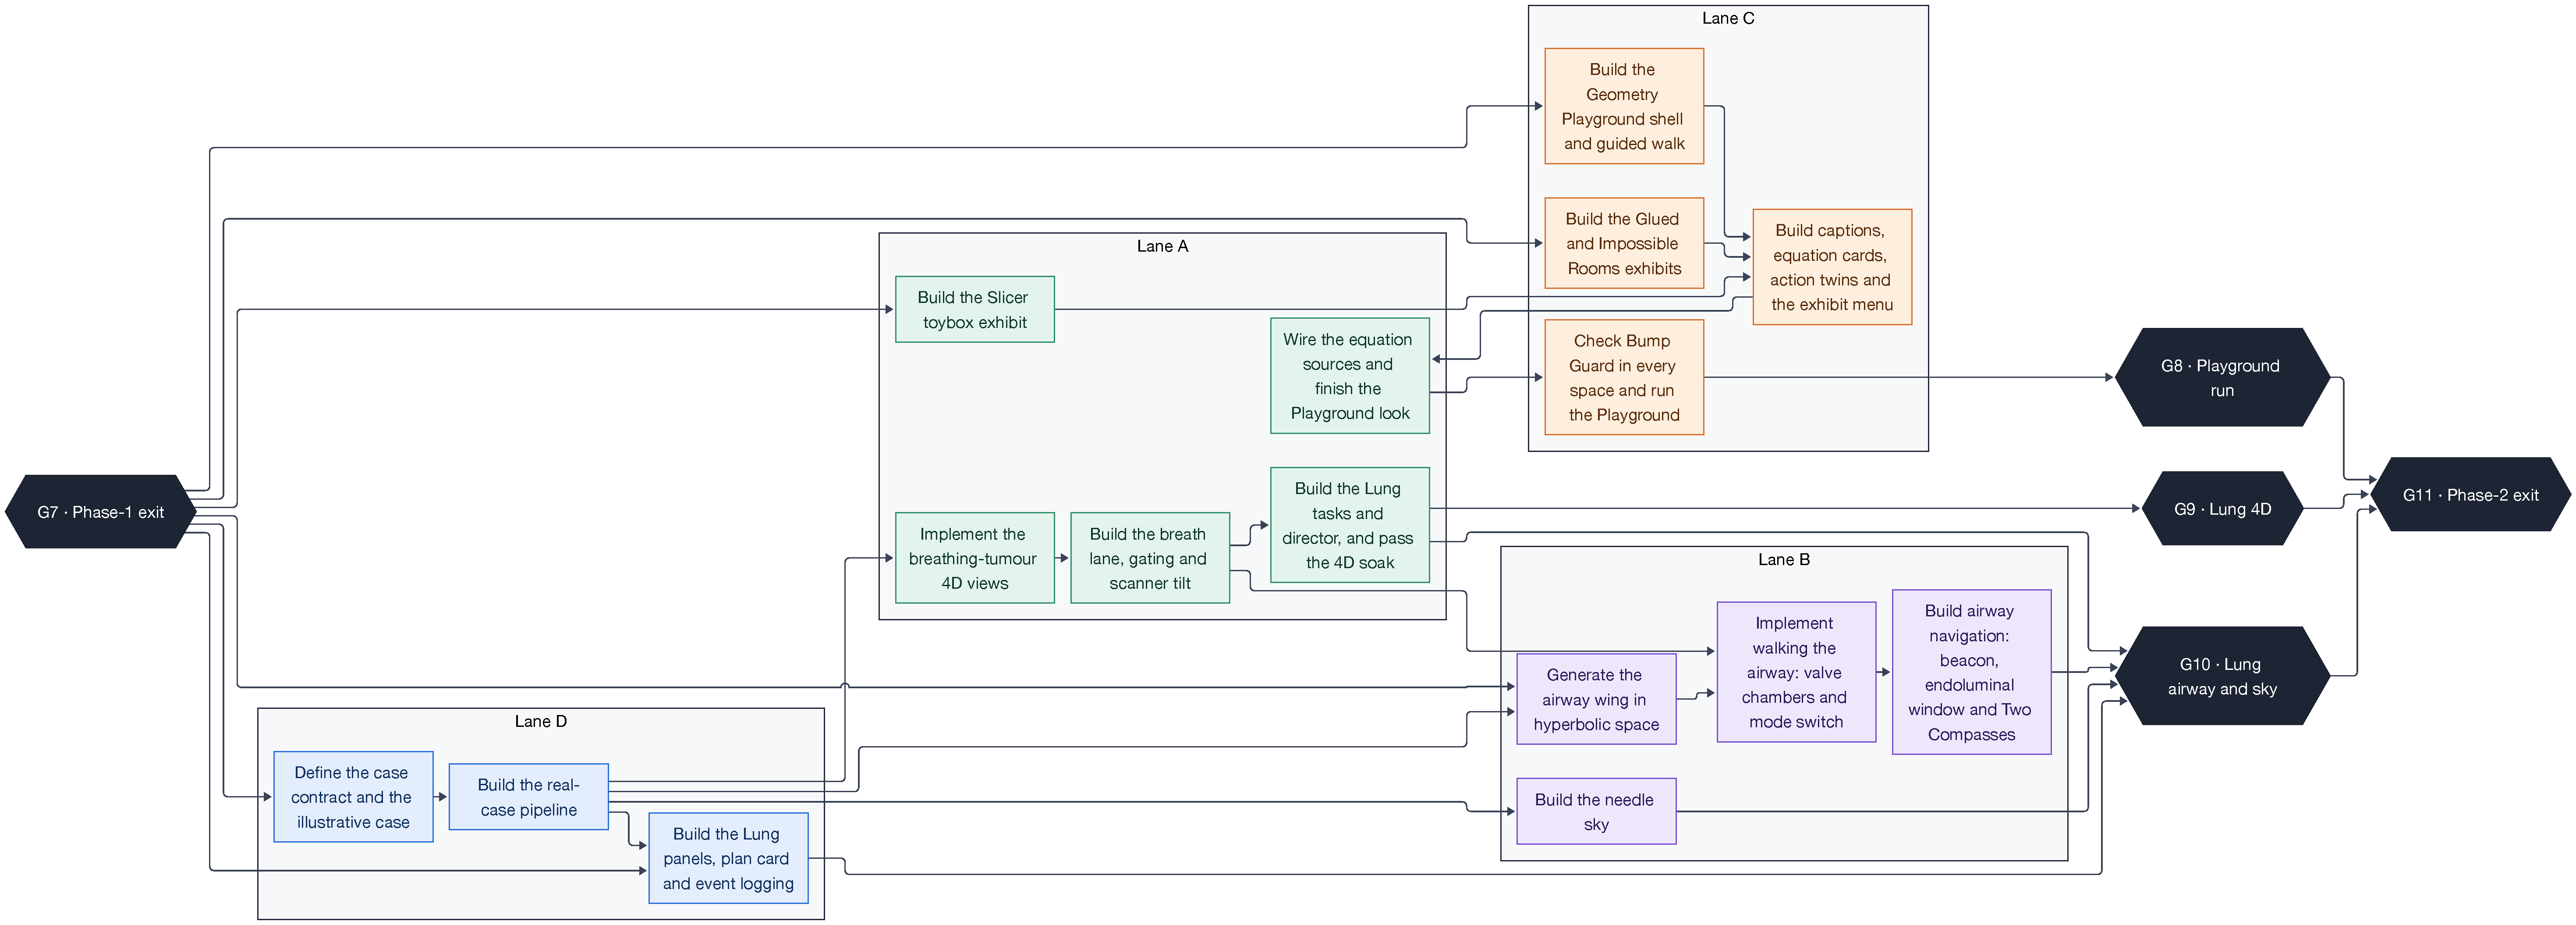
\includegraphics[width=392mm,height=215mm,keepaspectratio]{figures/build_graph/phase2_areas.pdf}}
\medskip
\figcap{Colours: green lane A, purple lane B, orange lane C, blue lane D; dark hexagons are gates. Each box shows the name of the area; what it covers is in the tables that follow.}
\end{bigpage}

\clearpage
\sub{The areas, lane by lane}{}
\lanetitle{Lane A · Platform, Look and Flat Spaces}
\begin{areatable}
  \tg{A}{A1} \textbf{Build the Slicer toybox exhibit}\newline the Slicer toybox with section names and shadow
  & \none{nothing in this phase}
  & \none{--}
  & \tg{C}{C2} Slicer toybox
  & \none{--}
  & \ids{2 tasks: P2-A01, A02} \\ \thinrule
  \tg{A}{A2} \textbf{Wire the equation sources and finish the Playground look}\newline the live numbers behind the equation cards of the exhibits, and the look polish of the Playground
  & \tg{A}{A1} \tg{C}{C3}
  & \tg{C}{C2} Caption chips and equation cards
  & \tg{C}{C4} Look polish; Exhibit equation sources
  & \none{--}
  & \ids{2 tasks: P2-A03, A04} \\ \thinrule
  \tg{A}{A3} \textbf{Implement the breathing-tumour 4D views}\newline the 4D tube loaded into Mesh4D, live slices with phase colouring, shells and the look-down shadow, the breathing chest, and the ring fallback
  & \tg{D}{D1}
  & \tg{D}{D2} atlas case chest
  & \none{--}
  & \none{--}
  & \ids{6 tasks: P2-A20, A21, A22, A23, A24, A30} \\ \thinrule
  \tg{A}{A4} \textbf{Build the breath lane, gating and scanner tilt}\newline the breath lane with the unroll animation and "now" plane, the gating flags, and the scanner tilt
  & \tg{A}{A3}
  & \none{--}
  & \tg{B}{B2} Unroll animation and "now" plane
  & \none{--}
  & \ids{4 tasks: P2-A25, A26, A27, A28} \\ \thinrule
  \tg{A}{A5} \textbf{Build the Lung tasks and director, and pass the 4D soak}\newline tasks M2, M3 and M4 with scoring and events, the Lung director with labels and credits, and the Lung 4D soak report
  & \tg{A}{A4}
  & \tg{D}{D2} atlas case pack and delivery
  & \none{--}
  & \gate{G9} \gate{G10}
  & \ids{3 tasks: P2-A29, A31, A32} \\ \thinrule
\end{areatable}

\lanetitle{Lane B · Kernel and Curved Worlds}
\begin{areatable}
  \tg{B}{B1} \textbf{Generate the airway wing in hyperbolic space}\newline the airway tree mapped onto the tile graph, and the corridor and chamber kit
  & \none{nothing in this phase}
  & \tg{D}{D2} atlas case airway
  & \none{--}
  & \none{--}
  & \ids{2 tasks: P2-B01, B02} \\ \thinrule
  \tg{B}{B2} \textbf{Implement walking the airway: valve chambers and mode switch}\newline the valve solver for Mode 1, the valve walk for Mode 2, the mode switch, and the lesion chamber hand-over
  & \tg{B}{B1}
  & \tg{A}{A4} Unroll animation and "now" plane
  & \none{--}
  & \gate{G10}
  & \ids{4 tasks: P2-B03, B04, B05, B09} \\ \thinrule
  \tg{B}{B3} \textbf{Build airway navigation: beacon, endoluminal window and Two Compasses}\newline the beacon and route cost, the endoluminal window, Two Compasses, and the airway run test
  & \tg{D}{D2}
  & \tg{B}{B1} AirwayTree\newline \tg{B}{B2} Mode switch
  & \none{--}
  & \gate{G10}
  & \ids{4 tasks: P2-B06, B07, B08, B12} \\ \thinrule
  \tg{B}{B4} \textbf{Build the needle sky}\newline the needle sky with its phase and robust layers, and the great-circle check
  & \tg{D}{D2}
  & \none{--}
  & \none{--}
  & \gate{G10}
  & \ids{2 tasks: P2-B10, B11} \\ \thinrule
\end{areatable}

\lanetitle{Lane C · Scan, Room and Safety}
\begin{areatable}
  \tg{C}{C1} \textbf{Build the Geometry Playground shell and guided walk}\newline the director and beats, scan-to-Home, the centre mark and dial hand-off, the guided 3-4-5 walk, the mode compare, tutorial prompts with the comfort question, and the pointing probe
  & \none{nothing in this phase}
  & \none{--}
  & \none{--}
  & \none{--}
  & \ids{7 tasks: P2-C01, C02, C03, C04, C05, C09, C17} \\ \thinrule
  \tg{C}{C2} \textbf{Build captions, equation cards, action twins and the exhibit menu}\newline caption chips and equation cards, the action twins, and the exhibit menu with return to Home
  & \tg{C}{C1}
  & \tg{A}{A1} Slicer toybox\newline \tg{C}{C3} Glued exhibit: wrap-walk; Impossible Rooms exhibit
  & \tg{A}{A2} Caption chips and equation cards
  & \none{--}
  & \ids{3 tasks: P2-C06, C07, C08} \\ \thinrule
  \tg{C}{C3} \textbf{Build the Glued and Impossible Rooms exhibits}\newline the Glued exhibit with the chiral kit and the gluing switch, and the Impossible Rooms exhibit with the loop corridor
  & \none{nothing in this phase}
  & \none{--}
  & \tg{A}{A2} Glued exhibit: wrap-walk; Impossible Rooms exhibit; Chiral kit; Gluing switch and T³; Loop corridor and room numbers
  & \none{--}
  & \ids{5 tasks: P2-C12, C13, C14, C15, C16} \\ \thinrule
  \tg{C}{C4} \textbf{Check Bump Guard in every space and run the Playground}\newline the Bump Guard check repeated in every space, and the complete Playground run
  & \tg{A}{A2}
  & \tg{C}{C1} Scan-to-Home; Mode compare; Tutorial prompts and FMS; Pointing probe and SEQ\newline \tg{C}{C2} Action twins; Exhibit menu and return Home
  & \none{--}
  & \gate{G8}
  & \ids{2 tasks: P2-C10, C11} \\ \thinrule
\end{areatable}

\lanetitle{Lane D · Link, Station and Forge}
\begin{areatable}
  \tg{D}{D1} \textbf{Define the case contract and the illustrative case}\newline the case contract with its readers, and the illustrative case package that lanes A and B build against
  & \none{nothing in this phase}
  & \none{--}
  & \tg{A}{A3} Case contract; atlas case twin
  & \none{--}
  & \ids{2 tasks: P2-D01, D02} \\ \thinrule
  \tg{D}{D2} \textbf{Build the real-case pipeline}\newline the \code{atlas case} steps from fetch and masks to the 4D tube, shells, chest, airway and sky, packed and delivered to the phone
  & \tg{D}{D1}
  & \none{--}
  & \tg{A}{A3} atlas case chest\newline \tg{A}{A5} atlas case pack and delivery\newline \tg{B}{B1} atlas case airway\newline \tg{B}{B3} atlas case airway\newline \tg{B}{B4} atlas case sky
  & \none{--}
  & \ids{7 tasks: P2-D03, D04, D05, D06, D07, D08, D09} \\ \thinrule
  \tg{D}{D3} \textbf{Build the Lung panels, plan card and event logging}\newline the Lung Console panel, the Lung twins on Spectator and Console, the plan card, and event logging with the pilot export
  & \none{nothing in this phase}
  & \tg{D}{D1} Case contract\newline \tg{D}{D2} atlas case airway
  & \none{--}
  & \gate{G10}
  & \ids{4 tasks: P2-D10, D11, D12, D13} \\ \thinrule
\end{areatable}

\sub{Gates of this phase}{§9.4}
\begin{gatetable}
  \gate{G8} \textbf{Playground run} & \tg{C}{C4} Check Bump Guard in every space and run the Playground\newline \gate{G7} & A first-time walker completes the guided run in two different rooms & A, C, two first-time users \\ \thinrule
  \gate{G9} \textbf{Lung 4D} & \tg{A}{A5} Build the Lung tasks and director, and pass the 4D soak\newline \gate{G7} & The four 4D pieces run on both case packages at budget & A, B, D \\ \thinrule
  \gate{G10} \textbf{Lung airway and sky} & \tg{A}{A5} Build the Lung tasks and director, and pass the 4D soak\newline \tg{B}{B2} Implement walking the airway: valve chambers and mode switch\newline \tg{B}{B3} Build airway navigation: beacon, endoluminal window and Two Compasses\newline \tg{B}{B4} Build the needle sky\newline \tg{D}{D3} Build the Lung panels, plan card and event logging\newline \gate{G7} & Four forks walked without rescue; sky and plan card correct & B, D \\ \thinrule
  \gate{G11} \textbf{Phase-2 exit} & \gate{G8} \gate{G9} \gate{G10} & Playground and Lung Mission in one session by an outsider, hot, at budget & all four lanes \\ \thinrule
\end{gatetable}

\sub{What the plan says about this phase}{§9.6}
\begin{quoted}
Two tracks run in parallel from G7. The specifications and the work-package tables are in §10.1 (Playground) and §10.2 (Lung Mission); the diagrams here show the order.\par

{\tablefont\renewcommand{\arraystretch}{1.3}\setlength{\tabcolsep}{2mm}\begin{tabularx}{\linewidth}{@{}>{\RaggedRight\arraybackslash}X >{\RaggedRight\arraybackslash}X >{\RaggedRight\arraybackslash}X >{\RaggedRight\arraybackslash}X@{}}
\rowcolor{panel}\textbf{Track} & \textbf{Lanes} & \textbf{Packages} & \textbf{Exit gate} \\ \thickrule
Geometry Playground & C (shell; Glued and Impossible Rooms exhibits) and A (Slicer toybox, equation sources, look) & \code{P2-\allowbreak{}C01}–\code{P2-\allowbreak{}C17}, \code{P2-\allowbreak{}A01}–\code{P2-\allowbreak{}A04} & G8 \\ \thinrule
Lung Mission & D (Station pipeline, case packages, plan card), A (medical 4D runtime), B (airway wing, needle sky) & \code{P2-\allowbreak{}D01}–\code{P2-\allowbreak{}D13}, \code{P2-\allowbreak{}A20}–\code{P2-\allowbreak{}A32}, \code{P2-\allowbreak{}B01}–\code{P2-\allowbreak{}B12} & G9 (4D), G10 (airway and sky) \\ \thinrule
\end{tabularx}\par}

Lane A serves both tracks, which departs from a strict "two lanes each" (open item 17 in §14): the Slicer toybox and the medical 4D runtime both build on lane A's \code{Mesh4D}. Lane A does \code{P2-\allowbreak{}A01} and \code{P2-\allowbreak{}A02} first, because \code{P2-\allowbreak{}A01} unblocks lane C's exhibit menu (\code{P2-\allowbreak{}C08}), then starts \code{P2-\allowbreak{}A20} onwards; \code{P2-\allowbreak{}A03} and \code{P2-\allowbreak{}A04} follow when their lane-C inputs land.\par

What is sequential:\par

\begin{itemize}
  \item In the Playground everything hangs off the director (\code{P2-\allowbreak{}C01}); the exhibits wrap Phase 1 spaces and are independent of one another; the run (\code{P2-\allowbreak{}C11}) is last.
  \item In the Lung Mission the case contract (\code{P2-\allowbreak{}D01}) comes first. Lane D then produces the \textbf{illustrative} package (\code{P2-\allowbreak{}D02}) before the real one, so lanes A and B have data to build against without waiting for the full pipeline. The 4D runtime (lane A) and the airway wing (lane B) are independent of each other until the lesion chamber hand-over (\code{P2-\allowbreak{}B09}). The Lung director (\code{P2-\allowbreak{}A32}) stubs the beats that belong to lanes B and D, so G9 does not wait for the airway.
  \item G11 needs G8, G9 and G10, and then one combined session by someone from outside the team.
\end{itemize}
\end{quoted}

%% ======================================================================
%% Phase 3 · Shared House and FieldFit
%% ======================================================================

\clearpage\sect{Phase 3 · Shared House and FieldFit}{§9.7}\label{sec:p3}

\sub{Who can work side by side}{}

\intro{This phase opens when \gate{G11} Phase-2 exit has passed. 9 areas cover the 28 tasks of this phase. Across a row: areas that can be worked on at the same point. Down a column: one person's order. An area sits in the first step in which part of it can begin; it is finished only when everything under \emph{after} and \emph{needs} has arrived.}

\begin{board}{4}
 & \lanehead{A}{Lane A · Platform, Look and Flat Spaces} & \lanehead{B}{Lane B · Kernel and Curved Worlds} & \lanehead{C}{Lane C · Scan, Room and Safety} & \lanehead{D}{Lane D · Link, Station and Forge} \\[1mm]
\step{1} &
  \card{A}{A1}{Implement the two-sheet house: sheets, door and flat-twin data}{} &
  \card{B}{B1}{Implement the FieldFit lens}{needs \tg{D}{D2}}\card{B}{B2}{Build the Blind-Spot Finder}{} &
  \card{C}{C1}{Scan the second room and fit the door}{} &
  \card{D}{D1}{Relay the peer and show the two-plan flat twin}{needs \tg{A}{A1}}\card{D}{D2}{Build the FieldFit presets and lens panel}{needs \tg{B}{B1}} \\[.6mm]
\step{2} &
  \card{A}{A2}{Load the second home and the visitor}{after \tg{A}{A1} \quad needs \tg{C}{C1}} &
   &
   &
  \card{D}{D3}{Build the heatmap and the search task, and run the FieldFit measurement}{after \tg{B}{B1} \quad needs \tg{B}{B2}\,\tg{D}{D2} \quad feeds \gate{G13}} \\[.6mm]
\step{3} &
   &
   &
  \card{C}{C2}{Make the Shared House safe and shared, and walk it}{after \tg{A}{A2} \quad needs \tg{C}{C1}\,\tg{D}{D1} \quad feeds \gate{G12}} &
   \\[.6mm]
\end{board}


\clearpage
\sub{The work areas, as the plan draws them}{§9.7}
An arrow from a gate into an area means work in that area can start at that gate; an arrow between areas means the second cannot be finished without the first.\par\medskip
\centerline{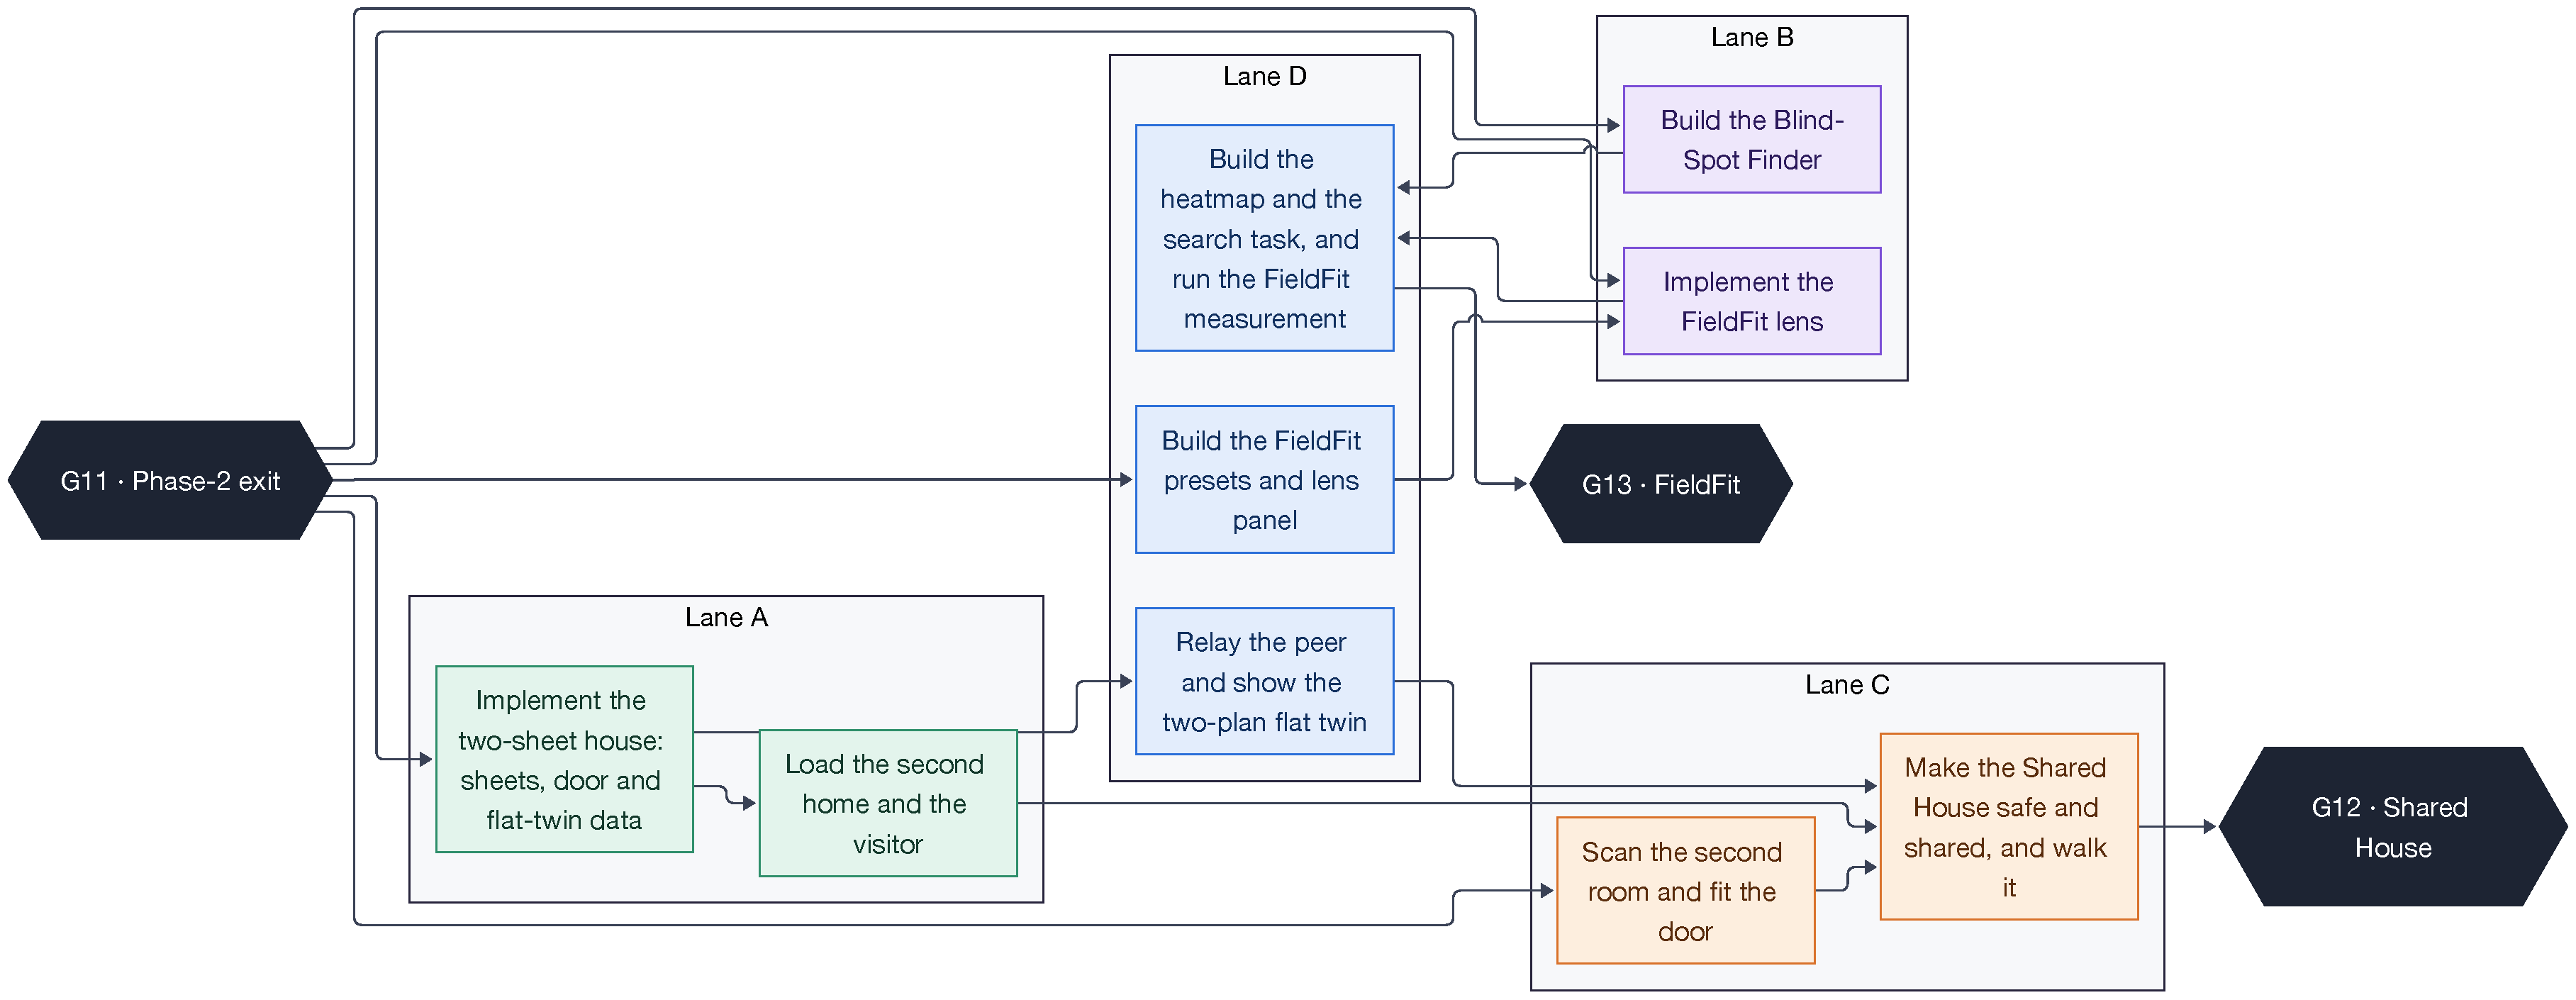
\includegraphics[width=\linewidth,height=120mm,keepaspectratio]{figures/build_graph/phase3_areas.pdf}}
\medskip
\figcap{Colours: green lane A, purple lane B, orange lane C, blue lane D; dark hexagons are gates. Each box shows the name of the area; what it covers is in the tables that follow.}

\clearpage
\sub{The areas, lane by lane}{}
\lanetitle{Lane A · Platform, Look and Flat Spaces}
\begin{areatable}
  \tg{A}{A1} \textbf{Implement the two-sheet house: sheets, door and flat-twin data}\newline the sheet state machine, the two-sheet door rendering, and the winding counter with the flat-twin data
  & \none{nothing in this phase}
  & \none{--}
  & \tg{D}{D1} Winding counter and flat-twin data
  & \none{--}
  & \ids{3 tasks: P3-A01, A02, A05} \\ \thinrule
  \tg{A}{A2} \textbf{Load the second home and the visitor}\newline the second home loader, the visitor avatar with its recorded track, the phone performance pass, and the guest rug if the lead approves it
  & \tg{A}{A1}
  & \tg{C}{C1} Door placement and door fit
  & \tg{C}{C2} Second home loader; Visitor avatar, recorded track, labels; Phone performance pass
  & \none{--}
  & \ids{4 tasks: P3-A03, A04, A06, A07} \\ \thinrule
\end{areatable}

\lanetitle{Lane B · Kernel and Curved Worlds}
\begin{areatable}
  \tg{B}{B1} \textbf{Implement the FieldFit lens}\newline the lens mathematics, the lookup builder, the wide source render with the composed final blit, the field-loss mask and slider, the lens guard, and the phone performance pass
  & \none{nothing in this phase}
  & \tg{D}{D2} Field presets
  & \tg{D}{D2} Lookup builder\newline \tg{D}{D3} Lens maths library; Field-loss mask and slider; Phone performance pass
  & \none{--}
  & \ids{6 tasks: P3-B01, B02, B03, B04, B05, B08} \\ \thinrule
  \tg{B}{B2} \textbf{Build the Blind-Spot Finder}\newline the Blind-Spot Finder, and Scotoma River (Extended)
  & \none{nothing in this phase}
  & \none{--}
  & \tg{D}{D3} Blind-Spot Finder
  & \none{--}
  & \ids{2 tasks: P3-B06, B07} \\ \thinrule
\end{areatable}

\lanetitle{Lane C · Scan, Room and Safety}
\begin{areatable}
  \tg{C}{C1} \textbf{Scan the second room and fit the door}\newline the second scan path, and door placement with the door fit
  & \none{nothing in this phase}
  & \none{--}
  & \tg{A}{A2} Door placement and door fit
  & \none{--}
  & \ids{2 tasks: P3-C01, C02} \\ \thinrule
  \tg{C}{C2} \textbf{Make the Shared House safe and shared, and walk it}\newline Bump Guard on the second sheet, the peer link (Extended), and the G12 walk-through
  & \tg{A}{A2}
  & \tg{C}{C1} Door placement and door fit\newline \tg{D}{D1} Peer relay (Extended); Two-plan flat twin
  & \none{--}
  & \gate{G12}
  & \ids{3 tasks: P3-C03, C04, C05} \\ \thinrule
\end{areatable}

\lanetitle{Lane D · Link, Station and Forge}
\begin{areatable}
  \tg{D}{D1} \textbf{Relay the peer and show the two-plan flat twin}\newline the peer relay (Extended) and the two floor plans with the winding dial on the Station
  & \none{nothing in this phase}
  & \tg{A}{A1} Winding counter and flat-twin data
  & \tg{C}{C2} Peer relay (Extended); Two-plan flat twin
  & \none{--}
  & \ids{2 tasks: P3-D07, D08} \\ \thinrule
  \tg{D}{D2} \textbf{Build the FieldFit presets and lens panel}\newline the field presets, the Console lens panel, and the Teichmüller lookup (Stretch)
  & \none{nothing in this phase}
  & \tg{B}{B1} Lookup builder
  & \tg{B}{B1} Field presets
  & \none{--}
  & \ids{3 tasks: P3-D01, D02, D05} \\ \thinrule
  \tg{D}{D3} \textbf{Build the heatmap and the search task, and run the FieldFit measurement}\newline the Spectator heatmap and bound, the search task with logging, and the G13 measurement run
  & \tg{B}{B1}
  & \tg{B}{B2} Blind-Spot Finder\newline \tg{D}{D2} Console lens panel
  & \none{--}
  & \gate{G13}
  & \ids{3 tasks: P3-D03, D04, D06} \\ \thinrule
\end{areatable}

\sub{Gates of this phase}{§9.4}
\begin{gatetable}
  \gate{G12} \textbf{Shared House} & \tg{C}{C2} Make the Shared House safe and shared, and walk it\newline \gate{G11} & Post Circling walked by three people with no contact & A, C, both phones \\ \thinrule
  \gate{G13} \textbf{FieldFit} & \tg{D}{D3} Build the heatmap and the search task, and run the FieldFit measurement\newline \gate{G11} & Blind spot found; search is faster with the lens than without & B, D \\ \thinrule
\end{gatetable}

\sub{What the plan says about this phase}{§9.7}
\begin{quoted}
Two independent use cases, two lanes each; lane D adds two small packages to the Shared House (the peer relay and the two-plan flat twin). Specifications and work-package tables: §10.3 and §10.4. Packages marked Extended, Stretch or Blocked are drawn but feed no gate.\par
\end{quoted}

%% ======================================================================
%% Phase 4 · Finish
%% ======================================================================

\clearpage\sect{Phase 4 · Finish}{§9.8}\label{sec:p4}

\sub{Who can work side by side}{}

\intro{This phase opens when \gate{G12} Shared House and \gate{G13} FieldFit have passed. 8 areas cover the 22 tasks of this phase. Across a row: areas that can be worked on at the same point. Down a column: one person's order. An area sits in the first step in which part of it can begin; it is finished only when everything under \emph{after} and \emph{needs} has arrived.}

\begin{board}{4}
 & \lanehead{A}{Lane A · Platform, Look and Flat Spaces} & \lanehead{B}{Lane B · Kernel and Curved Worlds} & \lanehead{C}{Lane C · Scan, Room and Safety} & \lanehead{D}{Lane D · Link, Station and Forge} \\[1mm]
\step{1} &
  \card{A}{A1}{Finish the look of every space and harden performance}{feeds \gate{G14}} &
  \card{B}{B1}{Prove and document the mathematics}{feeds \gate{G15}} &
  \card{C}{C1}{Polish onboarding and the pre-scan fast path}{feeds \gate{G15}} &
  \card{D}{D1}{Build the judges' dashboard and the session logs}{}\card{D}{D2}{Produce the metrics report, the video, the deck and the offline pack}{needs \tg{A}{A1}\,\tg{D}{D1} \quad feeds \gate{G15}} \\[.6mm]
\step{2} &
   &
   &
  \card{C}{C2}{Run the failure drills and the rehearsals}{after \tg{C}{C1} \quad needs \tg{D}{D1} \quad feeds \gate{G14}\,\gate{G15}}\card{C}{C3}{Write the comfort protocol, the sign and the briefings}{needs \gate{G14}\,\tg{D}{D1} \quad feeds \gate{G15}} &
   \\[.6mm]
\step{3} &
  \card{A}{A2}{Add audio, audit the comments and ship the golden build}{after \tg{A}{A1}\,\tg{C}{C2} \quad needs \gate{G14} \quad feeds \gate{G15}} &
   &
   &
   \\[.6mm]
\end{board}


\begin{bigpage}{Phase 4 · Finish}
\sub{The work areas, as the plan draws them}{§9.8}
An arrow from a gate into an area means work in that area can start at that gate; an arrow between areas means the second cannot be finished without the first.\par\medskip
\centerline{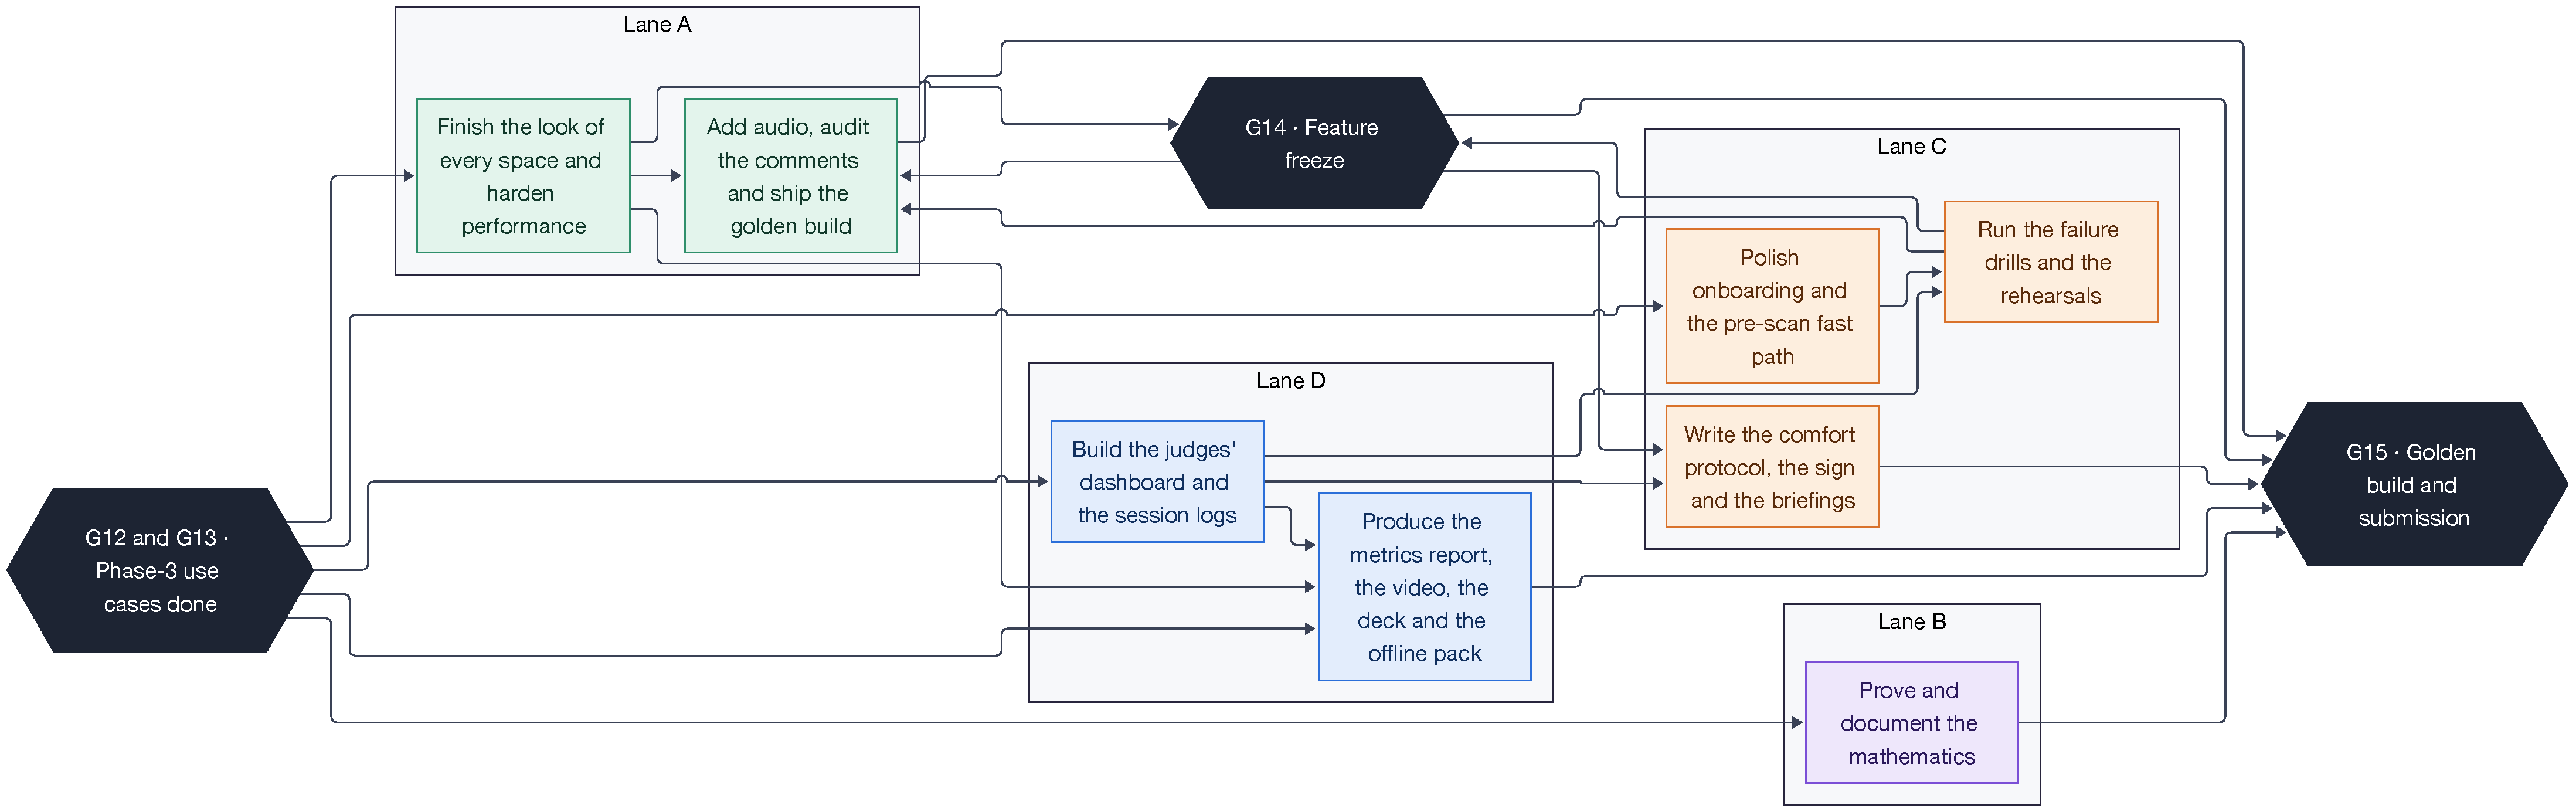
\includegraphics[width=392mm,height=215mm,keepaspectratio]{figures/build_graph/phase4_areas.pdf}}
\medskip
\figcap{Colours: green lane A, purple lane B, orange lane C, blue lane D; dark hexagons are gates. Each box shows the name of the area; what it covers is in the tables that follow.}
\end{bigpage}

\clearpage
\sub{The areas, lane by lane}{}
\lanetitle{Lane A · Platform, Look and Flat Spaces}
\begin{areatable}
  \tg{A}{A1} \textbf{Finish the look of every space and harden performance}\newline the look pass for every space and the soak on both phones, which is what the feature freeze waits for
  & \none{nothing in this phase}
  & \none{--}
  & \tg{D}{D2} Performance hardening
  & \gate{G14}
  & \ids{2 tasks: P4-A01, A03} \\ \thinrule
  \tg{A}{A2} \textbf{Add audio, audit the comments and ship the golden build}\newline the audio loops and cues, the comment audit, and the golden build with its launch check
  & \tg{A}{A1} \tg{C}{C2}
  & \gate{G14}
  & \none{--}
  & \gate{G15}
  & \ids{3 tasks: P4-A02, A04, A05} \\ \thinrule
\end{areatable}

\lanetitle{Lane B · Kernel and Curved Worlds}
\begin{areatable}
  \tg{B}{B1} \textbf{Prove and document the mathematics}\newline the maths notes, the correctness report, the equation-card audit, the figure data, and the prior-art note
  & \none{nothing in this phase}
  & \none{--}
  & \none{--}
  & \gate{G15}
  & \ids{5 tasks: P4-B01, B02, B03, B04, B05} \\ \thinrule
\end{areatable}

\lanetitle{Lane C · Scan, Room and Safety}
\begin{areatable}
  \tg{C}{C1} \textbf{Polish onboarding and the pre-scan fast path}\newline onboarding polished with outside walkers, and the pre-scan fast-path drill
  & \none{nothing in this phase}
  & \none{--}
  & \none{--}
  & \gate{G15}
  & \ids{2 tasks: P4-C01, C03} \\ \thinrule
  \tg{C}{C2} \textbf{Run the failure drills and the rehearsals}\newline the failure drills and the rehearsals with outside walkers
  & \tg{C}{C1}
  & \tg{D}{D1} Judges' dashboard
  & \tg{A}{A2} Failure drills
  & \gate{G14} \gate{G15}
  & \ids{2 tasks: P4-C04, C05} \\ \thinrule
  \tg{C}{C3} \textbf{Write the comfort protocol, the sign and the briefings}\newline the comfort protocol, the booth sign and the spotter briefing
  & \none{nothing in this phase}
  & \gate{G14}\newline \tg{D}{D1} Session log and pilot data
  & \none{--}
  & \gate{G15}
  & \ids{2 tasks: P4-C02, C06} \\ \thinrule
\end{areatable}

\lanetitle{Lane D · Link, Station and Forge}
\begin{areatable}
  \tg{D}{D1} \textbf{Build the judges' dashboard and the session logs}\newline the judges' dashboard, and the session log with the pilot data
  & \none{nothing in this phase}
  & \none{--}
  & \tg{C}{C2} Judges' dashboard\newline \tg{C}{C3} Session log and pilot data
  & \none{--}
  & \ids{2 tasks: P4-D01, D02} \\ \thinrule
  \tg{D}{D2} \textbf{Produce the metrics report, the video, the deck and the offline pack}\newline the metrics report, the Spectator capture, the deck with its claims check, and the offline pack
  & \none{nothing in this phase}
  & \tg{A}{A1} Performance hardening\newline \tg{D}{D1} Session log and pilot data; Judges' dashboard
  & \none{--}
  & \gate{G15}
  & \ids{4 tasks: P4-D03, D04, D05, D06} \\ \thinrule
\end{areatable}

\sub{Gates of this phase}{§9.4}
\begin{gatetable}
  \gate{G14} \textbf{Feature freeze} & \tg{A}{A1} Finish the look of every space and harden performance\newline \tg{C}{C2} Run the failure drills and the rehearsals\newline \gate{G12} \gate{G13} & Full path twice in a row on one phone without cooling; only fixes after this & all four lanes \\ \thinrule
  \gate{G15} \textbf{Golden build and submission} & \tg{A}{A2} Add audio, audit the comments and ship the golden build\newline \tg{B}{B1} Prove and document the mathematics\newline \tg{C}{C1} Polish onboarding and the pre-scan fast path\newline \tg{C}{C2} Run the failure drills and the rehearsals\newline \tg{C}{C3} Write the comfort protocol, the sign and the briefings\newline \tg{D}{D2} Produce the metrics report, the video, the deck and the offline pack\newline \gate{G14} & Golden build runs with the Station unplugged; documents, video and metrics delivered & all four lanes \\ \thinrule
\end{gatetable}

\sub{What the plan says about this phase}{§9.8}
\begin{quoted}
Polish, evaluation, demo operations and documentation. Work-package table: §13.6. Feature freeze (G14) follows the look pass, the performance hardening and the failure drills; after it, only fixes, audio, documents and rehearsals. In the diagrams of §9.7 and §9.8 the start gate shows when a lane is free; the tables give the technical dependency (§9.4).\par
\end{quoted}

%% ======================================================================
%% Ground rules
%% ======================================================================

\clearpage\sect{Ground rules}{}\label{sec:rules}

\sub{How the plan is organised}{§9.1}
\begin{itemize}
  \item \textbf{By dependency, not by date.} Every task lists what it needs and what proves it is done. A task starts when its inputs exist. A phase ends when its exit gate passes.
  \item \textbf{Contracts first.} The start is wide: three set-up tasks and four sets of contract pages have no dependency, so every engineer and their agents have work from the first minute. They meet in gate G0, where the interfaces between lanes are frozen and stubbed. After that the four lanes do not wait for each other's code until the integration gates.
  \item \textbf{Editor first, phone last.} Only one Mac can build to the phones, so everything that can be proved in the Unity Editor or in a unit test is proved there. The phone is for acceptance.
  \item \textbf{Two levels.} People plan in \textbf{work areas}: sixteen in Phase 1, a handful per lane, each a piece one person owns (§9.5.2); later phases have one to three areas per lane and use case (§9.6–9.8). Agents work on \textbf{tasks}: each task fits one coding agent, touches one lane's files, and has a binary acceptance test with numbers.
  \item \textbf{The plan's tables and diagrams come from one data set.} The Phase 1 graph has 70 tasks and 166 dependency edges, checked to be free of cycles; the diagrams below are generated from the same data as the tables.
\end{itemize}

\sub{Shared resources and the rules that protect them}{§9.3}
\begin{multicols}{2}
\minihead{The build seat (one Mac).}

\begin{enumerate}
  \item Lane A's first jobs are the build chain (\code{P1-\allowbreak{}A02}, \code{P1-\allowbreak{}A13}) and the URP settings and the stereo rig (\code{P1-\allowbreak{}A03}, \code{P1-\allowbreak{}A04}). They take priority over every other lane-A task until G1 passes. Editor-only lane-A task \code{P1-\allowbreak{}A06} and the Editor part of \code{P1-\allowbreak{}A12} run alongside them as the graph in §9.5.5 allows.
  \item Everyone runs the Unity Editor on their own machine. Native code is wrapped so the Editor and the Station build compile without it.
  \item Device builds go out as a build train: one integration build at every gate, plus short on-request slots from a visible queue (who, branch, what is tested).
  \item Prefer iteration that needs no rebuild: live tuning from the Console, replay of recorded RoomModels and pose logs in the Editor, kernel and graph logic as EditMode tests.
  \item One bundle id and one signing account. A build signed by a different account cannot install over the existing one.
\end{enumerate}

\minihead{The two phones.}

\begin{enumerate}
  \item Phone A is the reference device for every published number. Phone B is lane C's working device (every one of lane C's Phase-1 tasks except the Editor-only FloorScan core, \code{P1-\allowbreak{}C15}, needs a phone), the hot-swap spare, and the second walker in Phase 3.
  \item Hand-held before head-mounted: scan, link and input are debugged with the phone in the hand; the headset is for acceptance.
  \item Record once, replay many times: the first good scan and a few walks are saved and replayed in the Editor by every lane.
  \item A soak leaves a phone hot. Soaks are scheduled, not squeezed between someone else's measurements, and the thermal state is noted at the start of every measurement.
\end{enumerate}

\textbf{The Station's GPU.} The RTX 5070 has 12 GB. The Forge's generator needs about 8 GB and owns the card while jobs are queued. The Spectator runs at modest settings beside it. The medical pipeline (\code{atlas case}, Phase 2) runs when the Forge is idle.\par

\textbf{Scenes and prefabs.} Unity scenes are single files, so each has exactly one owner.\par

{\tablefont\renewcommand{\arraystretch}{1.3}\setlength{\tabcolsep}{2mm}\begin{tabularx}{\linewidth}{@{}>{\RaggedRight\arraybackslash}X >{\RaggedRight\arraybackslash}X >{\RaggedRight\arraybackslash}X@{}}
\rowcolor{panel}\textbf{Asset} & \textbf{Owner} & \textbf{Rule} \\ \thickrule
\code{Atlas\_\allowbreak{}Boot} (XR origin, stereo rig, SpaceLab, bootstraps) & A & Nobody else edits it. Systems register themselves from their own scenes \\ \thinrule
\code{Space\_\allowbreak{}Home} & C & One additive scene per space, one owner each \\ \thinrule
\code{Space\_\allowbreak{}Glued}, \code{Space\_\allowbreak{}Portal}, \code{Space\_\allowbreak{}Slicer} & A &  \\ \thinrule
\code{Space\_\allowbreak{}CurvedWalk}, \code{Space\_\allowbreak{}AlignedCells}, \code{Space\_\allowbreak{}SmallPlanet} & B &  \\ \thinrule
\code{Sys\_\allowbreak{}Scan}, \code{Sys\_\allowbreak{}BumpGuard}, \code{Sys\_\allowbreak{}Onboarding} & C & Loaded additively by the boot scene \\ \thinrule
\code{Sys\_\allowbreak{}Link}, \code{Sys\_\allowbreak{}Hud}, \code{PC\_\allowbreak{}Spectator} & D & The Spectator scene is never in the iOS build list \\ \thinrule
Use-case scenes (Phase 2 onwards) & The lane that owns the use case's runtime & Reference spaces through \code{ISpaceModule}; never copy their objects \\ \thinrule
\code{Sandbox\_\allowbreak{}\textless{}name\textgreater{}} & Each engineer & Never in the build list \\ \thinrule
URP assets, Project Settings, layers, stencil table, package manifest & A & Changed only by A, announced first \\ \thinrule
The shared material and palette & A & Per-tile and per-room material instances are created at run time from a pool, never saved as assets \\ \thinrule
\end{tabularx}\par}

\textbf{The shared shader.} Ownership of the four include files is in §8.3. A contract check runs at every gate: the shader is still reported SRP-Batcher compatible, and the draw-call count of the stress scene has not grown.\par

\textbf{Source control.} Text serialisation, visible meta files, UnityYAMLMerge as the merge tool, Git LFS for binaries. Small merges to one main branch. Tunables live in the parameter registry and in ScriptableObjects, one file per space, so tuning never touches a scene. Asset Store packs stay out of the repository.\par
\end{multicols}

\clearpage\sub{Working with AI coding agents}{§9.9}
The tasks are sized and worded to be handed over. The rules that make that safe:\par

\begin{enumerate}
  \item \textbf{One task, one branch, one merge request.} The branch name is the task id.
  \item \textbf{An agent stays in its lane's folders.} It may read contracts and other lanes' public interfaces; it may not edit them. A contract change is made by a human and announced.
  \item \textbf{The acceptance test comes first.} For anything provable in the Editor the agent writes the test from the acceptance cell, sees it fail, then implements.
  \item \textbf{Parallel agents take tasks marked ‖} in §9.5.1: they touch different files by construction.
  \item \textbf{A human runs every phone test} and records the numbers. An agent prepares the build, the test scene and the checklist.
  \item \textbf{No agent merges on a red test or a broken shader contract.}
  \item \textbf{Numbers in a task are part of the task.} If a budget cannot be met, the agent reports the measured value and stops; it does not relax the number.
\end{enumerate}

A task brief, ready to paste:\par

\begin{Verbatim}[fontsize=\footnotesize,frame=none,xleftmargin=2mm]
Task        P1-B04  Exact tile ids and the tile graph            Lane B
Read first  docs/contracts/kernel.md; this plan §3.4, §6.5, Appendix A.5
Depends on  P1-B01 (merged)
You own     Assets/Atlas/Kernel/Tiling/**  and its tests. Touch nothing else.
Deliver     TileId.cs, TileGraph.cs, Tests/TileIdTests.cs
Accept      - per-depth tile counts equal OEIS A377322 to depth 10
            - a walk round a vertex closes after exactly 5 steps
            - φ(X²+Y²) − T² = −1 for every generated tile (evaluated in Int128)
            - tile centres within ρ = 2 / 3 / 3.5 / 4 of a tile centre: 13 / 45 / 81 / 129; within 3.8425: 105
            - a tile crossing costs ≤ 0.5 ms in the Editor
Out of scope  rendering, materials, scenes, shader code
Report      test log; measured crossing cost; anything in the contract you could not satisfy
\end{Verbatim}

\end{document}
